%
% exemplo genérico de uso da classe iiufrgs.cls
% $Id: iiufrgs.tex,v 1.1.1.1 2005/01/18 23:54:42 avila Exp $
%
% This is an example file and is hereby explicitly put in the
% public domain.
%
\documentclass[ecp,tc]{iiufrgs}
% Para usar o modelo, deve-se informar o programa e o tipo de documento.
% Programas :
%   * cic       -- Graduação em Ciência da Computação
%   * ecp       -- Graduação em Ciência da Computação
%   * ppgc      -- Programa de Pós Graduação em Computação
%   * pgmigro   -- Programa de Pós Graduação em Microeletrônica
%   
% Tipos de Documento:
%   * tc                -- Trabalhos de Conclusão (apenas cic e ecp)
%   * diss ou mestrado  -- Dissertações de Mestrado (ppgc e pgmicro)
%   * tese ou doutorado -- Teses de Doutorado (ppgc e pgmicro)
%   * ti                -- Trabalho Individual (ppgc e pgmicro)
% 
% Outras Opções:
%   * english    -- para textos em inglês
%   * openright  -- Força início de capítulos em páginas ímpares (padrão da
%                   biblioteca)
%   * oneside    -- Desliga frente-e-verso
%   * nominatalocal -- Lê os dados da nominata do arquivo nominatalocal.def

\newcommand*{\captionsource}[2]{%
  \caption[{#1}]{#1}\par
  \textbf{Fonte:} #2\par
}


% Use unicode
\usepackage[utf8]{inputenc}   % pacote para acentuação

% Necessário para incluir figuras
\usepackage{graphicx}           % pacote para importar figuras

% Multirow é usado pras tabelas
\usepackage{multirow}
% Float é usado pro [H] nas figuras
\usepackage{float}

\usepackage{times}              % pacote para usar fonte Adobe Times
% \usepackage{palatino}
% \usepackage{mathptmx}          % p/ usar fonte Adobe Times nas fórmulas

\usepackage[alf,abnt-emphasize=bf]{abntex2cite}	% pacote para usar citações abnt

%
% Informações gerais
%
\title{Um método para avaliação de desempenho de implementações \textit{open source} em software de núcleos de rede 5G}

\author{Lando}{Gabriel}
% alguns documentos podem ter varios autores:
%\author{Flaumann}{Frida Gutenberg}
%\author{Flaumann}{Klaus Gutenberg}

% orientador e co-orientador são opcionais (não diga isso pra eles :))
\advisor[Prof.~Dr.]{Wickboldt}{Juliano}
%\coadvisor[Prof.~Dr.]{Knuth}{Donald Ervin}

% a data deve ser a da defesa; se nao especificada, são gerados
% mes e ano correntes
%\date{maio}{2001}

% o local de realização do trabalho pode ser especificado (ex. para TCs)
% com o comando \location:
%\location{Itaquaquecetuba}{SP}

% itens individuais da nominata podem ser redefinidos com os comandos
% abaixo:
% \renewcommand{\nominataReit}{Prof\textsuperscript{a}.~Wrana Maria Panizzi}
% \renewcommand{\nominataReitname}{Reitora}
% \renewcommand{\nominataPRE}{Prof.~Jos{\'e} Carlos Ferraz Hennemann}
% \renewcommand{\nominataPREname}{Pr{\'o}-Reitor de Ensino}
% \renewcommand{\nominataPRAPG}{Prof\textsuperscript{a}.~Joc{\'e}lia Grazia}
% \renewcommand{\nominataPRAPGname}{Pr{\'o}-Reitora Adjunta de P{\'o}s-Gradua{\c{c}}{\~a}o}
% \renewcommand{\nominataDir}{Prof.~Philippe Olivier Alexandre Navaux}
% \renewcommand{\nominataDirname}{Diretor do Instituto de Inform{\'a}tica}
\renewcommand{\nominataCoord}{Prof.~Walter Fetter Lages}
% \renewcommand{\nominataCoordname}{Coordenador do PPGC}
% \renewcommand{\nominataBibchefe}{Beatriz Regina Bastos Haro}
% \renewcommand{\nominataBibchefename}{Bibliotec{\'a}ria-chefe do Instituto de Inform{\'a}tica}
% \renewcommand{\nominataChefeINA}{Prof.~Jos{\'e} Valdeni de Lima}
% \renewcommand{\nominataChefeINAname}{Chefe do \deptINA}
% \renewcommand{\nominataChefeINT}{Prof.~Leila Ribeiro}
% \renewcommand{\nominataChefeINTname}{Chefe do \deptINT}

% A seguir são apresentados comandos específicos para alguns
% tipos de documentos.

% Relatório de Pesquisa [rp]:
% \rp{123}             % numero do rp
% \financ{CNPq, CAPES} % orgaos financiadores

% Trabalho Individual [ti]:
% \ti{123}     % numero do TI
% \ti[II]{456} % no caso de ser o segundo TI

% Monografias de Especialização [espec]:
% \espec{Redes e Sistemas Distribuídos}      % nome do curso
% \coord[Profa.~Dra.]{Weber}{Taisy da Silva} % coordenador do curso
% \dept{INA}                                 % departamento relacionado

%
% palavras-chave
% iniciar todas com letras minúsculas, exceto no caso de abreviaturas
%
% \keyword{my5G-RANTester}
% \keyword{Núcleo 5G}
% \keyword{Teste de desempenho}
% \keyword{Redes móveis}
% \keyword{Open5GS}
% \keyword{free5GC}

\keyword{Redes móveis}
\keyword{Núcleo 5G}
\keyword{Teste de desempenho}
\keyword{\textit{Open5GS}}
\keyword{\textit{free5GC}}
\keyword{\textit{my5G-RANTester}}


%
% inicio do documento
%
\begin{document}

% folha de rosto
% às vezes é necessário redefinir algum comando logo antes de produzir
% a folha de rosto:
% \renewcommand{\coordname}{Coordenadora do Curso}
\maketitle

% dedicatoria
\clearpage
\begin{flushright}
\mbox{}\vfill
{\sffamily\itshape
``I wanna rock and roll all night\\
And party every day\\}
--- \textsc{Gene Simmons and Paul Stanley}
\end{flushright}

% agradecimentos
\chapter*{Agradecimentos}
Aos meus pais, Ernesto Antônio Lando e Izidora Justina Bizotto Lando, e à minha irmã, Anelise Lando, que me apoiaram, acreditaram em mim e me deram suporte desde que saí de casa para vir morar sozinho em outro Estado para cursar Engenharia de Computação em uma das melhores universidades do país. Muito obrigado.

À Isadora, minha parceira de vida, que esteve ao meu lado nesses últimos anos, me apoiando, incentivando e ouvindo eu reclamar de tudo.
Muito obrigado, Isa, por toda essa parceria, conselhos e ajuda que você me deu. Eu evoluí muito como pessoa ao seu lado.

Ao Felipe Lando, meu irmão, que me acolhe desde as tentativas falhas do vestibular da UFRGS até hoje, juntamente com a minha cunhada, Amália Machado.
Muito obrigado por todos esses anos de parceria, muitos almoços, jantas e projetos que fizemos juntos desde que eu vim morar na Capital.
À Amália, um agradecimento especial por toda a ajuda que você me deu durante o desenvolvimento deste trabalho.
Se eu estou aqui hoje é principalmente graças a vocês dois e a Acadêmica Pesquisa.

Ao Urso, meu cachorro, que esteve ao meu lado durante todo o desenvolvimento deste trabalho, seja me mordendo, latindo, pulando por cima de mim querendo brincar ou só deitado em silêncio me fazendo companhia.
Eu sei que você não entende a importância do que eu estava fazendo, mas muito obrigado pelo carinho.

Aos meus colegas de trabalho da HP, que compreenderam as diversas vezes que precisei me ausentar para poder realizar atividades referentes a este trabalho.
Aqui vai um agradecimento especial à Thayná Minuzzo, que além de colega de trabalho, também foi minha colega durante a graduação, me ajudando em diversas disciplinas, incluindo dicas durante a realização do presente trabalho.
Vocês também tem uma parte desta minha conquista. Muito obrigado.

Aos meus colegas e amigos que estão comigo desde a primeira semana de aula, como a Ana e a Narumi, o Fischer, o Probst e o Rodrigo, além de outras amizades que eu fiz durante todos esses anos de graduação.
Vocês me confortaram, muitas vezes indiretamente, só de saber que todos nós estávamos passando pelas mesmas dificuldades durante toda a graduação, incluindo nesse trabalho.

Aos meus padrinhos e primos, Tia Enedina, Tio Ronei, Leonardo, Ramon, Lucas e Marina, que sempre me incentivaram e me acolheram nos feriados e finais de semana.
Muito obrigado por esse tempo juntos, me ajudaram a esfriar a cabeça nos momentos mais difíceis da graduação.

Ao meu orientador, Prof. Dr. Juliano Wickboldt, que me ofereceu a primeira oportunidade de bolsa de pesquisa, lá em 2017, no meu segundo semestre de graduação, com o Projeto FUTEBOL e, em 2021, aceitou ser meu orientador para o desenvolvimento desta pesquisa.
Aqui também vão meus agradecimentos aos bolsistas de iniciação científica do projeto PORVIR-5G, Lucas Schierholt e Mateus Milesi, que me ajudaram no desenvolvimento deste trabalho.
Sem vocês, eu não teria chegado até aqui.

Por fim, agradeço a todos aqueles que, de alguma forma, contribuíram para que este trabalho fosse concluído.
Espero que os resultados obtidos ajudem a desenvolver essa área da computação.



% resumo na língua do documento
\begin{abstract}
O presente trabalho desenvolve uma prova de conceito de um módulo para execução de testes de desempenho em implementações de núcleos de redes 5G.
O objetivo deste trabalho é analisar como se comportam as diferentes implementações de código aberto dos núcleos de rede 5G, \textit{free5GC}, \textit{Open5GS} e \textit{OpenAirInterface}, para a execução de procedimentos em escala.
Para responder a esse problema, primeiramente foi feito um um breve resumo sobre a evolução das redes móveis, com foco em implementações em software de núcleos de redes 5G.
A seguir, são apresentados os trabalhos relacionados, assim como as diferenças entre eles e a presente pesquisa.
Após, uma arquitetura de software foi desenvolvida, criando um módulo de extensão para o testador \textit{my5G-RANTester} para realizar testes de desempenho nessas implementações de código aberto de núcleos de redes 5G.
Foram executados experimentos sobre essas implementações.
Na primeira fase dos experimentos, foi feito um teste para analisar o tempo médio de conexão de cada equipamento de usuário com cada núcleo testado. Na segunda etapa do experimento, foi medida a largura de banda do plano de dados entre o equipamento de usuário e o núcleo da rede.
Dentre os principais resultados obtidos, foi possível observar que o \textit{free5GC} apresenta melhor desempenho em relação à largura de banda disponível para os equipamentos de usuário, enquanto que o \textit{Open5GS} apresenta mais estabilidade durante o processo de registro de múltiplos equipamentos de usuário.
Este trabalho possui duas importantes contribuições teóricas para a literatura. A primeira contribuição é a agregação de conhecimento sobre testes de desempenho em redes móveis, enquanto a segunda é relacionada com a estabilidade e limitações das implementações de núcleos 5G em software.
A principal contribuição prática deste trabalho é o desenvolvimento de um módulo para realizar testes de desempenho em núcleos de rede 5G.
Como sugestões de futuras pesquisas, é possível avançar a investigação sobre experimentos em núcleos comerciais ou replicar os testes em ambientes de fácil escalabilidade.


\end{abstract}

% resumo na outra língua
% como parametros devem ser passados o titulo e as palavras-chave
% na outra língua, separadas por vírgulas
\begin{englishabstract}{A method for evaluating the performance of open source software implementations of 5G network cores}{Mobile networks. 5G core. Performance tests. Open5GS. free5GC. my5G-RANTester}
The present work develops a proof of concept of a module to run performance tests on 5G network core implementations.
The main goal of this work is to analyze how the different open source implementations of the 5G network cores behave, such as free5GC, Open5GS and OpenAirInterface, for the execution of procedures at scale.
To answer this problem, a brief summary of the evolution of mobile networks was made, focusing on software implementations of 5G network cores.
Next, the related works are presented, as well as the differences between them and the present research.
Afterwards, a software architecture was developed, creating an extension module for the my5G-RANTester to run performance tests on these open source implementations of 5G network cores.
Experiments were performed on these implementations.
In the first phase of the experiments, a test was carried out to analyze the average connection time of each user equipment with each tested core. In the second stage of the experiment, the data plane throughput between the user equipment and the network core was measured.
Among the main results obtained, it was possible to observe that free5GC presents better performance in relation to the throughput available to user equipments, while Open5GS presents more stability during the registration process of multiple user equipments.
This work has two important theoretical contributions to the literature. The first contribution is the aggregation of knowledge about performance testing in mobile networks, while the second is related to the stability and limitations of 5G core implementations in software.
The main practical contribution of this work is the development of a module to run performance tests on 5G network cores.
As suggestions for future research, it is possible to advance the investigation on experiments in commercial cores or to replicate the tests in easily scalable environments.
\end{englishabstract}

% lista de abreviaturas e siglas
% o parametro deve ser a abreviatura mais longa
\begin{listofabbrv}{Serving GW}
    \item[1G]       Primeira geração de redes móveis
    \item[2G]       Segunda geração de redes móveis
    \item[3G]       Terceira geração de redes móveis
    \item[3GPP]     \textit{3rd Generation Partnership Project}
    \item[4G]       Quarta geração de redes móveis
    \item[5G]       Quinta geração de redes móveis
    \item[5GC]      \textit{5G Core}
    \item[5GNR]     \textit{5G New Radio}
    \item[AF]       \textit{Application Function}
    \item[AMF]      \textit{Access and Mobility Management Function}
    \item[API]      \textit{Application Programming Interface}
    \item[AUSF]     \textit{Authentication Server Function}
    \item[Bps]      \textit{Bytes} por segundo
    \item[CN]       \textit{Core Network}
    \item[CPU]      \textit{Central Processing Unit}
    \item[eNodeB]   \textit{Evolved Node B}
    \item[EPC]      \textit{Evolved Packet Core}
    \item[E-UTRAN]  \textit{Evolved UTRAN}
    \item[Gbps]     Giga \textit{bits} por segundo
    \item[gNB]      \textit{gNodeB}
    \item[GSM]      \textit{Global System for Mobile Communications}
    \item[HSDPA]    \textit{High-Speed Downlink Packet Access}
    \item[HSS]      \textit{Home Subscriber Server}
    \item[IoT]      \textit{Internet of Things}
    \item[IP]       \textit{Internet Protocol}
    \item[kbps]     Quilo \textit{bits} por segundo
    \item[KVM]      \textit{Kernel-based Virtual Machine}
    \item[LTE]      \textit{Long Term Evolution}
    \item[LTE-A]    \textit{LTE-Advanced}
    \item[LTE-R]    \textit{LTE-Railway}
    \item[Mbps]     Mega \textit{bits} por segundo
    \item[MME]      \textit{Mobility Management Entity}
    \item[MQTT]     \textit{Message Queuing Telemetry Transport}
    \item[ms]       Milissegundos
    \item[N3IWF]    \textit{Non-3GPP InterWorking Function}
    \item[NAS]      \textit{Non-Access Stratum}
    \item[NB]       \textit{Node B}
    \item[NEF]      \textit{Network Exposure Function}
    \item[NGAP]     \textit{NG Application Protocol}
    \item[NRF]      \textit{Network Repository Function}
    \item[ns]       Nanossegundos
    \item[NSA]      \textit{Non-Stand Alone}
    \item[NSSF]     \textit{Network Slice Selection Function}
    \item[NWDAF]    \textit{Network Data Analytics Function}
    \item[OAI]      \textit{OpenAirInterface}
    \item[PCF]      \textit{Policy Control Function}
    \item[PDN GW]   \textit{Packet Data Network Gateway}
    \item[PDU]      \textit{Packet Data Unit}
    \item[PORVIR-5G] \textit{Programmability, Orchestration and Virtualization on 5G networks}
    \item[PSTN]     \textit{Public Switched Telephone Network}
    \item[QoS]      Qualidade de serviço
    \item[RAN]      \textit{Radio Access Network}
    \item[s]        Segundos
    \item[SA]       \textit{Stand Alone}
    \item[SBA]      \textit{Service-based Architecture}
    \item[Serving GW]  \textit{Serving Gateway}
    \item[SMF]      \textit{Session Management Function}
    \item[SMS]      \textit{Short Message Service}
    \item[TCP]      \textit{Transmission Control Protocol}
    \item[UDM]      \textit{Unified Data Management}
    \item[UDP]      \textit{User Datagram Protocol}
    \item[UE]       \textit{User Equipment}
    \item[UMTS]     \textit{Universal Mobile Telecommunications System}
    \item[UPF]      \textit{User Plane Function}
    \item[UTRAN]    \textit{UMTS Terrestial Radio Network}
    \item[VoIP]     \textit{Voice over IP}
    \item[VoLTE]    \textit{Voice over LTE}
    \item[WCDMA]    \textit{Wide-Band Code-Divison Multiple Access}
\end{listofabbrv}

% idem para a lista de símbolos
%\begin{listofsymbols}{$\alpha\beta\pi\omega$}
%       \item[$\sum{\frac{a}{b}}$] Somatório do produtório
%       \item[$\alpha\beta\pi\omega$] Fator de inconstância do resultado
%\end{listofsymbols}

% lista de figuras
\listoffigures

% lista de tabelas
\listoftables

% sumario
\tableofcontents

% aqui comeca o texto propriamente dito

% introducao
\chapter{Introdução}
\label{chap:intro}
A quinta geração de redes móveis (5G) teve sua especificação inicial disponibilizada em 2017 na \textit{Release 15} da \textit{3rd Generation Partnership Project} (3GPP) \cite{Redana2020}, trazendo diversas melhorias em relação à quarta geração de redes móveis (4G).
É possível citar como principais melhorias da 5G em relação às gerações anteriores as maiores taxas de transferência de dados, a maior área de cobertura, a menor latência de comunicação, o suporte à maior densidade de dispositivos e a redução no consumo de energia \cite{Ahmad2019}.

Para que seja possível atingir as metas propostas, uma reformulação no núcleo da rede se torna necessária por ser considerado o elemento mais crítico da 5G \cite{Cardoso2020}.
O núcleo de uma rede 5G é responsável por estabelecer uma conexão estável e segura entre dispositivos e prover acesso aos serviços disponibilizados pela rede móvel.

Com o objetivo de reduzir os custos de implantação e manutenção das redes móveis, iniciou-se o desenvolvimento de implementações em software do seu núcleo.
Implementações em software desse componente permitem que atualizações sejam feitas de forma simplificada, possibilitando a correção de falhas descobertas durante a operação da rede. Além disso, facilita a evolução da rede para futuras gerações, sem a necessidade de realizar deslocamento para os locais de instalação dos equipamentos, visto que a atualização pode ser feita de forma remota.
O hardware utilizado para a implantação dessas redes em software é um equipamento de propósito geral, fabricado em larga escala e com custos reduzidos.

A implementação de redes móveis privadas, sem vínculo com operadoras, se tornou uma opção para simplificar a implantação de redes sem fios em larga escala em ambientes corporativos, principalmente pela facilidade de implementação em máquinas convencionais.
O conceito de redes móveis privadas surgiu com o advento da Indústria 4.0, que visa transformar a manufatura industrial por meio da digitalização e exploração das potencialidades das novas tecnologias \cite{Rojko2017}.
Uma indústria pode criar e gerenciar sua própria rede 4G ou 5G, permitindo a conexão de milhares de dispositivos e sensores, provendo segurança, performance e baixa latência.
Existem implementações \textit{open source} em software de estações de rádio e núcleos de redes 4G e 5G, como \textit{free5GC}\footnote{\url{https://www.free5gc.org}}, \textit{Open5GS}\footnote{\url{https://open5gs.org}}, \textit{OpenAirInterface}\footnote{\url{https://openairinterface.org}} (OAI), \textit{srsRAN}\footnote{\url{https://www.srslte.com}}, dentre outras, facilitando a implantação desse tipo de rede móvel em ambientes corporativos.

Uma vez que deseja-se implementar uma rede móvel privada, é preciso avaliar o cenário para identificar a melhor relação custo-benefício.
Sendo assim, é preciso verificar, principalmente, a área de cobertura a ser atendida pelas antenas, quantos dispositivos serão conectados, qual o tráfego de dados que será gerado e qual a latência máxima desejada para a comunicação dos dispositivos.
Após coletar essas informações, pode-se definir o tipo de equipamento que precisa ser adquirido para suprir a necessidade dessa rede.
Entretanto, para que se possa definir qual o hardware a ser usado, é preciso saber como as implementações \textit{open source} se comportam ao serem executadas nesses equipamentos.

Nesse contexto, estão inseridos os testes para averiguar o comportamento dessas redes móveis em diversos cenários.
Como as implementações \textit{open source} não possuem garantias, é preciso executar testes de conformidade e robustez, por exemplo, para garantir que o núcleo da rede se comporte da forma que foi especificado.
Além disso, é preciso aferir o desempenho das diversas implementações, permitindo avaliar qual hardware seria capaz de rodar a implementação desejada de acordo com a capacidade da rede que se deseja implementar.

Desta forma, o presente trabalho tem como objetivo responder a seguinte questão: como se comportam as diferentes implementações \textit{open source} de núcleo 5G para execução dos procedimentos em escala?
Esse trabalho aplica o teste de desempenho nos núcleos de rede 5G \textit{free5GC}, \textit{Open5GS} e OAI. Para isso, é proposta e implementada uma arquitetura através de um módulo de extensão do testador \textit{my5G-RANTester}\footnote{https://github.com/my5G/my5G-RANTester} para executar testes de desempenho sobre essas implementações de núcleo 5G.

Quanto às contribuições teóricas, este trabalho agrega conhecimento em relação a testes de desempenho, sobretudo em núcleos de redes 5G, trazendo discussões relevantes para a área de desenvolvimento de software.
Também apresenta as limitações encontradas nas implementações testadas, mostrando a maturidade dessas implementações para uso em escala.
Em relação às contribuições práticas, este trabalho desenvolve um módulo para ser acoplado em um testador de código aberto de núcleos de rede 5G.

Sendo assim, o trabalho foi dividido nos seguintes capítulos.
O capítulo de fundamentação teórica descreve a evolução das redes móveis e traz definições sobre testes em software.
No capítulo de trabalhos relacionados, é descrito os trabalhos que se assemelham com o presente trabalho, além de demonstrar o que este trabalho difere da literatura atual.
O capítulo de solução demonstra a arquitetura desenvolvida para execução de experimentos de testes de desempenho, coleta e análise de dados.
No capítulo de análise dos dados coletados, é discutido os resultados dos experimentos, demonstrando o desempenho e as limitações encontradas nos núcleos testados.
Por fim, nas considerações finais, é apresentado com mais detalhes as contribuições teóricas e práticas, as limitações encontradas e sugestões de futuros trabalhos a partir destas descobertas.


\chapter{Fundamentação teórica}
\label{chap:background}
\section{Primeiras gerações de redes móveis}

Devido à complexidade das redes móveis modernas, conhecer a evolução dessas redes se torna necessário para facilitar o seu entendimento. Originalmente, as redes móveis tinham o foco em comunicações de voz analógica, sendo uma extensão da rede de telefonia pública \textit{(Public Switched Telephone Network - PSTN)}, que operava com rede de roteamento de circuitos \cite{Cardoso2020}.
Entretanto, essas redes móveis foram adaptadas para transporte de dados com taxas de transmissão muito baixas, atingindo velocidades de até 2.4 kbps. Essas redes ficaram conhecidas como rede móvel de primeira geração (1G) \cite{vora2015evolution}.

Com a necessidade de evoluir as redes 1G, surge a segunda geração (2G), que provia um sinal com melhor qualidade, maiores taxas de transferência de dados e maior aproveitamento do espectro das ondas de rádio.
Todavia, essa tecnologia ainda mantinha seu foco em roteamento de circuitos.
Nessa geração, também surge o serviço de troca de mensagens curtas, conhecido como \textit{Short Message Service} (SMS).
Foi no 2G que a tecnologia de transporte de dados \textit{Global System for Mobile Communications} (GSM) foi inserida \cite{bhalla2010generations}.

Em 1998, inicia-se a parceria entre diversas organizações responsáveis pela criação dos padrões de telecomunicação denominada 3GPP\footnote{\url{https://www.3gpp.org/about-3gpp}}, que publica a \textit{Release 1999} no início do ano 2000.
Em redes móveis, \textit{releases} são conjuntos de recursos e especificações disponibilizadas a cada período, definindo os padrões a serem seguidos para a implementação dessas redes.
A \textit{Release 1999} descreve uma nova tecnologia de redes móveis, com foco em roteamento de pacotes.
Porém, essa tecnologia mantinha a compatibilidade com as tecnologias antigas, sendo denominada redes móveis de terceira geração (3G) \cite{3gpp.01.01}.

Inicialmente, o padrão definido para as redes 3G foi o \textit{Wide-Band Code-Divison Multiple Access} (WCDMA).
Entretanto, em 2002, o início do desenvolvimento do padrão \textit{High-Speed Downlink Packet Access} (HSDPA) é anunciado, suportando velocidades de transmissão teóricas de até 14 Mbps. Isso permitiria navegação na internet mais rápida, acesso a conteúdos de televisão diretamente no aparelho celular e chamadas de vídeo. O padrão HSDPA foi chamado de 3.5G e teve a sua especificação finalizada em 2004 \cite{Lamba2012}.

No final de 2008, a \textit{Release 8} é publicada pela 3GPP, especificando os requisitos para a tecnologia \textit{Long Term Evolution} (LTE), que viria para substituir a terceira geração de redes móveis.
Entretanto, essa especificação não preenchia os requisitos mínimos para ser considerada uma quarta geração de redes móveis, sendo assim conhecida como 3.9G \cite{delperal2018}.
Dentre as mudanças provindas desta nova tecnologia, é importante mencionar a remoção do suporte à roteamento de circuitos, fazendo com que essa geração usasse apenas roteamento de pacotes sobre IP para todo o tráfego de informações na rede.

Toda a informação de áudio de ligações telefônicas era trafegada sobre a rede de roteamento de circuitos nas gerações anteriores ao LTE.
Com a remoção dessa tecnologia no LTE, foi necessário desenvolver um novo protocolo, surgindo assim o \textit{Voice over LTE} (VoLTE).
O VoLTE, assim como a tecnologia \textit{Voice over IP} (VoIP), trafega os dados de voz de ligações telefônicas sobre a rede de roteamento de pacotes, permitindo que as operadoras de redes móveis pudessem continuar oferecendo o serviço de ligações telefônicas para seus clientes. Nesta época, esse serviço era o mais rentável para as operadoras \cite{Yi2012}. 

Visando preencher os requisitos mínimos para a criação da quarta geração de redes móveis (4G), no início de 2011 é publicada a \textit{Release 10} pela 3GPP, criando assim a tecnologia \textit{LTE-Advanced} (LTE-A) \cite{3gpp.21.201}.
O 4G prometia velocidades de \textit{download} de pico de até 1Gbps e velocidades de \textit{upload} de pico de até 100Mbps.
Atingir tais velocidades só era possível graças à remoção do suporte ao roteamento de circuitos que ocorreu no 3.9G.

Antes do surgimento do LTE, existiam apenas 3 componentes na rede. Um era o equipamento de usuário, denominado \textit{User Equipment} (UE), sendo esse o dispositivo móvel. Outro componente era a rede de acesso via rádio, ou \textit{Radio Access Network} (RAN), denominada na tecnologia 3G de \textit{Universal Mobile Telecommunications System (UMTS) Terrestial Radio Network} (UTRAN), que englobava a estação de rádio base, chamada de \textit{Node B} (NB). Por fim, o terceiro componente era o núcleo da rede, ou \textit{Core Network} (CN), que no 3G era denominado \textit{UMTS Core Network} \cite{Miah2002}.
No entanto, a especificação da rede LTE trouxe uma melhor separação dos seus componentes do núcleo da rede, denominado \textit{Evolved Packet Core} (EPC) nessa geração, além de renomear a RAN para \textit{Evolved UTRAN} (E-UTRAN), chamando a estação base de \textit{Evolved Node B} (eNodeB).
O EPC foi separado em 4 elementos, sendo eles o \textit{Serving Gateway (Serving GW)}, o \textit{Packet Data Network Gateway (PDN GW)}, o \textit{Mobility Management Entity} (MME) e o \textit{Home Subscriber Server} (HSS) \cite{3gpp.23.214}.

\section{Redes 5G}

Em 2017, a 3GPP publica a versão inicial da \textit{Release 15}, com as definições da quinta geração de redes móveis, o 5G \cite{3gpp.21.205}.
Assim como nas gerações anteriores, o 5G visava introduzir melhorias na capacidade de transmissão de dados da RAN e redução da latência de comunicação entre o UE e a RAN.
Entretanto, essa geração teve como objetivo criar uma rede mais dinâmica e com maior flexibilidade em relação ao LTE.
Nessa geração também houve a integração com tecnologias de comunicação sem fios não-3GPP, que enquadram dispositivos denominados de \textit{Internet of Things} (IoT).

A \textit{Release 15} também introduziu as arquiteturas de rede 5G \textit{Non-Stand Alone} (NSA) e 5G \textit{Stand Alone} (SA).
Na arquitetura NSA, o núcleo da rede 4G é utilizado para a autenticação e comunicação dos dispositivos 5G, substituindo-se a E-UTRAN pela \textit{5G New Radio} (5GNR) e, consequentemente, a eNodeB pela gNodeB.
A rede NSA é considerada uma rede de transição entre o 4G e o 5G, pois o custo de implementação é baixo em ambientes onde já existe cobertura 4G das operadoras.

Por outro lado, a arquitetura SA introduziu um novo núcleo da rede, denominado de \textit{5G Core} (5GC).
De acordo com a especificação da 3GPP, o 5GC é um conjunto de componentes interconectados através de uma camada de serviços. Cada componente tem seu grupo específico de responsabilidades por consumir e prover serviços de e para outros elementos do sistema 5G, através de uma \textit{Application Programming Interface} (API).

A quinta geração de redes móveis também trouxe uma nova arquitetura do núcleo da rede, ilustrada em alto nível na Figura \ref{fig:5Gcore}. Os principais componentes dessa rede são o \textit{Access and Mobility Management Function} (AMF), o \textit{Session Management Function} (SMF) e o \textit{User Plane Function} (UPF).
O AMF é responsável por garantir que o processo de comunicação ocorra de maneira coesa e transparente, considerando a mobilidade do usuário como principal fator.
O SMF é responsável por estabelecer, modificar e liberar as sessões de cada equipamento de usuário, além de requisitar a alocação de um endereço de IP para esses UEs.
O UPF é o responsável pelo processamento e encaminhamento dos dados provindos dos UEs. Esses componentes serão discutidos com maior profundidade na subseção \ref{sub:components}.

\begin{figure}[!ht]
    \centering
    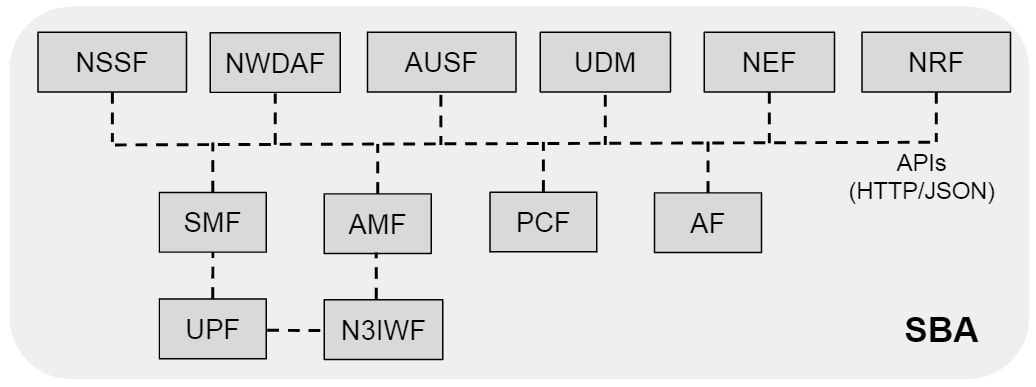
\includegraphics[width=1\textwidth]{TG2/Chapters/Background/Figures/Background-Core5G.png}
    \captionsource{Core 5G software components.}{\cite[p.~15]{Cardoso2020}}
    \label{fig:5Gcore}
\end{figure}

Os demais nove componentes do núcleo do 5G realizam uma variedade de funções.
O \textit{Authentication Server Function} (AUSF) é a função responsável por prover os serviços de autenticação dos UEs.
O \textit{Unified Data Management} (UDM) gerencia as informações dos usuários conectados na rede.
O \textit{Network Repository Function} (NRF) é um repositório que lista todas as funções de rede disponíveis em sua instância do núcleo do 5G.
O \textit{Policy Control Function} (PCF) é o responsável por controlar o comportamento da rede, aplicando políticas de segurança e controle.
O \textit{Network Slice Selection Function} (NSSF) é o componente responsável por controlar os \textit{slices} da rede para cada UE.
O \textit{Network Exposure Function} (NEF) é responsável por expor eventos internos relacionados aos UEs.
O \textit{Network Data Analytics Function} (NWDAF) é a função responsável por coletar e analisar dados provindos dos outros componentes da rede, incluindo informações dos usuários.
O \textit{Application Function} (AF) é um componente genérico que interage com os outros componentes no intuito de melhorar a qualidade do serviço para o usuário.
O \textit{Non-3GPP InterWorking Function} (N3IWF) é o responsável por integrar dispositivos não-3GPP com a rede 5G.

\subsection{Protocolos NAS e NGAP e Sessões de PDU}

Os protocolos \textit{Non-Access Stratum} (NAS) e \textit{NG Application Protocol} (NGAP) são essenciais para a comunicação entre o núcleo da rede, a RAN e o UE através do plano de controle.
As sessões de \textit{Packet Data Unit} (PDU) são importantes para garantir o funcionamento do plano de usuário da rede 5G.
A Figura \ref{fig:5Gprotocols} representa a arquitetura de uma rede 5G, exibindo os protocolos NAS e NGAP e as sessões de PDU entre o equipamento de usuário, a gNodeB e o núcleo da rede.

\begin{figure}[!ht]
    \centering
    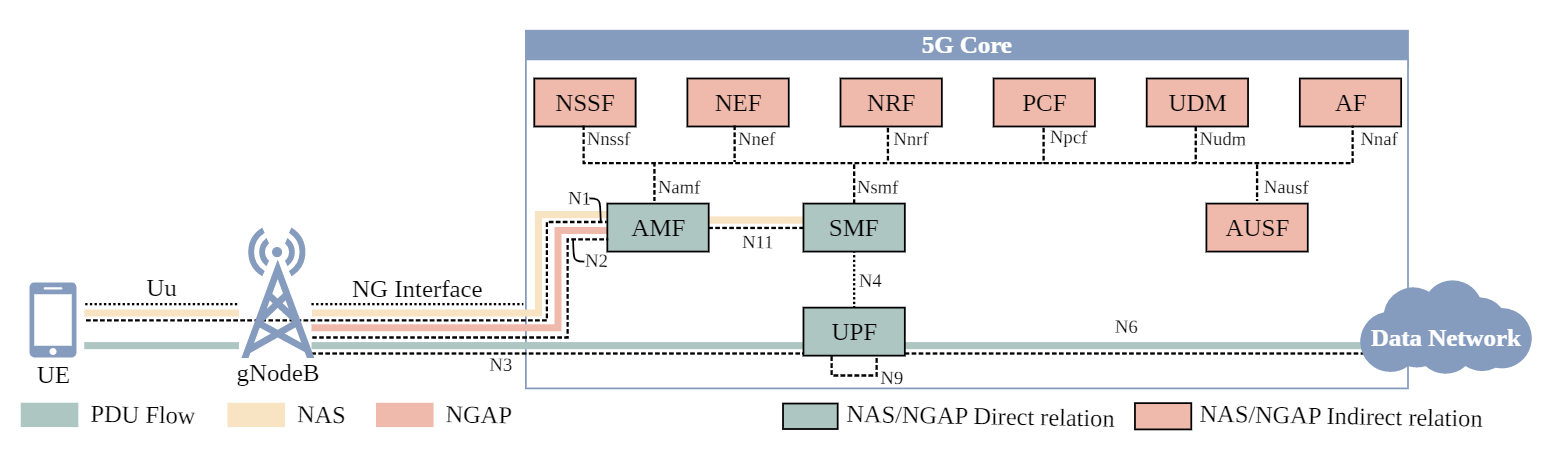
\includegraphics[width=1\textwidth]{TG2/Chapters/Background/Figures/Background-5GSystemProtocols.png}
    \captionsource{5G Core (5GC) Service-based Architecture (SBA).}{\cite[p.~3]{Dominato2021}}
    \label{fig:5Gprotocols}
\end{figure}

O protocolo NAS é usado para fazer a comunicação entre o UE e a função do núcleo AMF, tanto para dispositivos 3GPP quanto não-3GPP. A principal função do protocolo NAS é dar suporte à mobilidade do equipamento de usuário, incluindo procedimentos como autenticação, identificação e atualização das configurações genéricas do UE. O NAS também é responsável por suportar os procedimentos de gerenciamento de sessões, para estabelecer e manter a conexão de dados entre o UE e a rede de dados \cite{3gpp.24.501}. Esse protocolo também é o responsável por fazer a autenticação e gerenciar a conexão da gNodeB com o núcleo da rede.

O protocolo NGAP é o protocolo padrão para a comunicação do plano de controle entre a RAN e o núcleo da rede. O NGAP suporta os procedimentos de gerenciamento de interfaces, transporte das mensagens do protocolo NAS, gerenciamento de contexto do UE e das sessões de PDU. O gerenciamento de interfaces é o responsável por estabelecer e manter a conexão entre os componentes do núcleo da rede, onde as mensagens dos protocolos NAS e NGAP são transportados. O Protocolo NGAP é responsável por encapsular e transportar as mensagens NAS, provindas do UE, entre a RAN e o AMF. O gerenciamento de contexto do UE provê informações dos UEs para a RAN, como informações de segurança, lista de restrições de mobilidade e capacidade do rádio do UE. O gerenciamento das sessões de PDU é responsável por gerenciar os fluxos das unidades de pacotes de dados entre o núcleo da rede e a RAN, estabelecendo a interface de rádio utilizada para tráfego de controle e dados dos UEs \cite{3gpp.38.413}.

As sessões de PDU são responsáveis por prover a conexão fim-a-fim para o plano de usuário entre o UE e a rede de dados externa, através da função de rede UPF.
O fluxo de dados trafegado através das sessões de PDU é chamado de fluxo PDU e seus pacotes de dados são encapsulando sobre o protocolo de rede \textit{User Datagram Protocol} (UDP) \cite{3gpp.38.415}.

\subsection{Principais componentes da Rede 5G}
\label{sub:components}

Dentro do núcleo da rede, os componentes AMF, SMF e UPF são os responsáveis por gerenciar todo o tráfego de informações provindos da RAN.
O AMF é a porta de entrada do núcleo da rede em relação ao plano de controle.
Sendo assim, todo o tráfego dos protocolos NAS e NGAP provindos da RAN é direcionado para essa função do núcleo da rede.
Quando uma nova gNodeB inicia o processo de conexão com um núcleo existente, a autenticação e o estabelecimento da conexão é feito através de mensagens trocadas que utilizam o protocolo NAS entre a RAN e o AMF.
Após estabelecida a conexão, uma mensagem é enviada da RAN para o SMF, indiretamente através do AMF, utilizando o protocolo NAS, para que o SMF tenha conhecimento da gNodeB e possa gerenciar sua sessão.

Estando a RAN operacional, dispositivos 3GPP e não-3GPP dentro da área de cobertura da antena poderão iniciar sua conexão com essa rede 5G. Um dispositivo 3GPP, ao iniciar a conexão com essa rede 5G, troca mensagens com a RAN através do protocolo NAS. A RAN encapsula essas mensagens para o protocolo NGAP e encaminha para o núcleo da rede. O AMF, comunicando-se com os demais componentes da rede, autentica o UE através de um fluxo de informações definido na \textit{Release 15} do 3GPP \cite{3gpp.29.509}. Após concluir a autenticação do UE, o SMF se torna o responsável por gerenciar a sessão do equipamento de usuário. Um fluxo de dados PDU é estabelecido entre o UE e a função do núcleo UPF, que é responsável por gerenciar e encaminhar os pacotes de dados provindos dos UEs.

O UPF é a função do núcleo da rede 5G responsável por ser o ponto de conexão do núcleo da rede com qualquer rede externa.
É o UPF que encaminha os pacotes de dados provindos do UE através das sessões de PDU para a rede externa, sendo o responsável pelo roteamento de pacotes entre a rede externa e os diversos UEs conectados nessa rede 5G.
Essa função do núcleo da rede 5G aloca os endereços de IP para os UEs quando requisitado pelo SMF \cite{3gpp.23.501}.
O UPF também é responsável por coletar métricas de qualidade de serviço (QoS) do plano de usuário que serão usadas na função NWDAF \cite{3gpp.23.548}.

\section{Testes em rede móveis definidas por software}

Segundo \cite[p.~2, tradução nossa]{Bertolino2003}, ``teste de software consiste na verificação dinâmica do comportamento de um programa em um conjunto finito de casos de teste, adequadamente selecionados do domínio de execuções geralmente infinitas, em relação ao comportamento esperado especificado".
Com relação ao comportamento das redes sem fios implementadas em software, é importante executar testes para garantir que o funcionamento da rede esteja dentro do esperado.
Dentre os tipos de testes que podem ser executados em cima de implementações de redes 5G \textit{open source}, os que se destacam são os testes de conformidade, robustez e desempenho, como descrito em \cite{Dominato2021} e \cite{Zhang2019ASO}.

\subsection{Testes de Conformidade}

De acordo com \cite{Sarikaya1989}, teste de conformidade é definido como a atividade de teste realizada com o objetivo de verificar as capacidades e o comportamento de uma implementação em teste em relação aos requisitos de conformidade fornecidos no padrão de protocolo.
Os resultados dos testes de conformidade são do tipo lógico, sendo verdadeiro no caso onde a implementação em teste seja aprovada e falso no caso contrário.
Dessa forma, o uso de testes de conformidade em redes 5G é importante para verificar se a implementação da rede móvel se comporta de acordo com a especificação da 3GPP em casos onde o equipamento de usuário execute corretamente as operações descritas.

\cite{Rayner1987} divide o grupo de testes de conformidade em quatro categorias: testes básicos de interconexão, testes de capacidade, testes de comportamento e testes de resolução de conformidade.
Os testes básicos de interconexão são feitos para detectar quaisquer casos graves de não conformidade com a especificação do sistema.
Os testes de capacidade verificam se as capacidades observáveis da implementação em teste estão de acordo com os requisitos de conformidade estática da especificação. Os testes de conformidade estática são executados sobre o código fonte da aplicação.
Os testes de comportamento verificam a implementação da forma mais abrangente possível para ver se a implementação está de acordo com os requisitos de conformidade dinâmica da especificação. Os testes de conformidade dinâmica são realizados durante ou após a execução da implementação.
Os testes de resolução de conformidade examinam em profundidade requisitos específicos na implementação, verificando se a implementação se comporta exatamente como a especificação destes requisitos.

\subsection{Testes de Robustez}

Segundo \cite[p.~64, tradução nossa]{IEEE.Standard.Glossary}, robustez é definida como ``o grau em que um sistema ou componente pode funcionar corretamente na presença de entradas inválidas ou condições ambientais estressantes".
Os resultados dos testes de robustez também são do tipo lógico, sendo verdadeiro no caso onde a implementação em teste seja aprovada e falso no caso contrário.
Sendo assim, o teste de robustez no núcleo de redes móveis verifica o comportamento da rede em situações atípicas. \cite{Dominato2021} dividem o grupo de testes de robustez em um subgrupo de testes, que envolve testes de registro, de autenticação e de segurança, além de testes específicos para cada protocolo e função de rede do núcleo que serão detalhados na Subseção \ref{subsec:Dominato}.

\subsection{Testes de Desempenho}

Os testes de desempenho são importantes para validar o funcionamento da rede em uma carga alta de trabalho, o que representa uma situação de sobrecarga de uso da rede, o que pode causar mal funcionamento da rede e, em situações mais críticas, uma interrupção total do serviço.
Para a execução de testes de desempenho, costuma-se usar aplicações de referência, chamados de \textit{benchmarks}.
Os \textit{softwares} de \textit{benchmark} são aqueles que utilizam os mesmos parâmetros de entrada para avaliar o desempenho de diferentes sistemas ou serviços \cite{Boano2018}.
Sendo assim, o usuário pode comparar as métricas obtidas na execução com métricas coletadas de outras execuções em diferentes sistemas ou serviços e avaliar o desempenho do teste.

Para a avaliação dos testes de desempenho em redes móveis em software, \cite{Lee2021} utilizam dois grupos de métricas.
O primeiro grupo engloba métricas de desempenho de rede: taxa de transferência de dados, latência e perda de pacotes.
O segundo grupo é composto por métricas de desempenho de \textit{hardware}: carga do processador, tempo de execução e tempo de processador.

Em relação as métricas de desempenho de rede, a taxa de transferência é definida por \cite[p.~77, tradução nossa]{IEEE.Standard.Glossary} como ``a quantidade de trabalho que pode ser realizada por um sistema ou componente de computador em um determinado período de tempo''. Sendo assim, a taxa de transferência de dados em uma rede pode ser caracterizada como a quantidade de dados movida com sucesso de um lugar para outro em um determinado período de tempo.
\cite[p.~43, tradução nossa]{IEEE.Standard.Glossary} definem latência como ``o intervalo de tempo entre o instante em que uma unidade de controle de instrução emite uma chamada de dados e o instante em que a transferência de dados é iniciada.'' Se tratando de redes de computadores, latência se refere ao tempo que um pacote de dados leva para ser gerado no emissor, transmitido pela rede, e recebido e decodificado no receptor.
\cite{Bhadra2015} definem perda de pacotes como a falha de pacotes de dados ao chegar a um destino específico. Esse tipo de falha tende a afetar os mais diversos tipos de comunicação e podem produzir dados incorretos no destinatário.

Quanto a métricas de desempenho do \textit{hardware}, a carga do processador, também conhecido como \textit{Central Processing Unit} (CPU), é definida como o número de processos que estão sendo executados por uma CPU ou estão aguardando para serem executados \cite{Sebastian2014}.
\cite[p.~242, tradução nossa]{Patterson2014-qv} definem tempo de execução como ``o tempo total necessário para o computador concluir uma tarefa, incluindo acessos ao disco, acessos à memória, atividades de entrada e saída de dados, sobrecarga do sistema operacional, tempo de execução da CPU e assim por diante''. Já o tempo de processador é definido como somente o tempo que a CPU gasta computando uma tarefa específica \cite{Patterson2014-qv}.


\chapter{Trabalhos relacionados}
\label{chap:related}
Nesta seção, são analisados alguns estudos publicados que apresentam testes em redes móveis.
A Tabela \ref{tab:related-works} mostra um resumo dos trabalhos relacionados.

% Please add the following required packages to your document preamble:
% \usepackage{graphicx}
\begin{table}[H]
\centering
\caption{Tabela comparando os trabalhos relacionados}
\label{tab:related-works}
\resizebox{\columnwidth}{!}{%
\begin{tabular}{lllll}
\hline
\multicolumn{1}{c}{\textbf{Autor}} &
  \multicolumn{1}{c}{\textbf{\begin{tabular}[c]{@{}c@{}}Tecnologias\\ testadas\end{tabular}}} &
  \multicolumn{1}{c}{\textbf{\begin{tabular}[c]{@{}c@{}}Tipos de\\ teste\end{tabular}}} &
  \multicolumn{1}{c}{\textbf{\begin{tabular}[c]{@{}c@{}}Códigos\\ testados\end{tabular}}} &
  \multicolumn{1}{c}{\textbf{\begin{tabular}[c]{@{}c@{}}Protocolos\\ testados\end{tabular}}} \\ \hline
\citeonline{Dominato2021} &
  5G &
  \begin{tabular}[c]{@{}l@{}}Conformidade\\ e robustez\end{tabular} &
  \textit{\begin{tabular}[c]{@{}l@{}}free5GC,\\ Open5GS\\ e OAI\end{tabular}} &
  NAS e NGAP \\ \hline
\citeonline{Lee2021} &
  5G &
  \begin{tabular}[c]{@{}l@{}}Conformidade\\ e desempenho\end{tabular} &
  \textit{free5GC} &
  Fluxo PDU \\ \hline
\begin{tabular}[c]{@{}l@{}}Garcia, Alfredsson and\\ Brunstrom (2015)\end{tabular} &
  \begin{tabular}[c]{@{}l@{}}HSDPA+\\ e LTE\end{tabular} &
  Desempenho &
  Não se aplica &
  Fluxo PDU \\ \hline
\citeonline{Boano2018} &
  IoT &
  Desempenho &
  Não se aplica &
  Não se aplica \\ \hline
\citeonline{MahnSuk2018} &
  LTE-R &
  Desempenho &
  Não se aplica &
  Não se aplica \\ \hline
\end{tabular}%
}
\end{table}

\section{\textit{Tutorial on communication between access networks and the 5G core}}
\label{sec:Dominato}

O estudo publicado por \citeonline{Dominato2021} cria uma prova de conceito de uma aplicação para testar núcleos \textit{open source} de rede 5G.
Para esse estudo, foram escolhidos os grupos de testes de conformidade e robustez.
As implementações suportadas por esse testador são \textit{free5GC}, \textit{Open5GS} e \textit{OAI}.

Essa prova de conceito simula uma RAN e um ou mais UEs.
O objetivo do estudo é analisar o comportamento dos diferentes núcleos de rede 5G em dois diferentes cenários.
O primeiro cenário executa ações de acordo com o que foi especificado pela 3GPP, através de testes de conformidade.
O segundo cenário executa ações utilizando informações inválidas, forçando o núcleo da rede a contornar essa situação de acordo com o especificado, o que representa os testes de robustez.

Em relação aos testes de conformidade, são executados 11 diferentes testes, sendo eles teste de registro, autenticação primária e estabelecimento de chave, identificação, transporte, modo de segurança, atualização de configuração genérica do UE, gerenciamento de sessão, gerenciamento de interface, transporte de mensagens NAS, gerenciamento de contexto do UE e gerenciamento de sessão do PDU.
Foi utilizada a \textit{Release 16} do 3GPP como base para a execução dos testes.
O núcleo \textit{Open5GS} foi aprovado em todos os testes de conformidade, enquanto que o \textit{OAI} e o \textit{free5GC} não responderam de acordo com a especificação no teste de atualização de configuração genérica do UE.

Em relação aos testes de robustez, foram executados 7 testes, sendo eles teste de registro, autenticação, segurança, seleção SMF, seleção UPF, validação do fluxo NAS e gerenciamento de interface.
No teste de registro, dois casos foram avaliados. No primeiro caso, o UE enviou uma requisição de registro sem o identificador do UE, que é um campo mandatório. No segundo caso, o UE enviou a requisição com as informações criptografadas.
No teste de autenticação, são realizadas duas operações incorretas. O primeiro teste foi realizado enviando informações inválidas como resposta no fluxo de autenticação, enquanto que o segundo teste foi forçando uma falha de sincronização entre o núcleo e o UE.
Para o teste de segurança, foram testadas duas configurações de segurança inválidas, sendo elas responder a uma solicitação de segurança sem enviar um parâmetro obrigatório na resposta e responder à solicitação sem retransmitir as informações de segurança da requisição.
Os teste de seleção SMF e seleção UPF representam um UE fazendo uma requisição para estabelecer um fluxo PDU, porém enviando informações mandatórias inválidas.
O teste de validação do fluxo NAS visa verificar se o núcleo da rede se comporta da forma esperada caso a requisição de estabelecimento de sessão PDU seja realizada enviando as informações necessárias em uma ordem incorreta.
Por fim, o teste de gerenciamento de interface simula o registro de uma nova RAN na rede 5G, porém enviando informações inválidas para o AMF, o qual deve rejeitar essa requisição. 

O estudo considera que todos os núcleos testados obtiveram um desempenho satisfatório para a operação dentro da normalidade. Entretanto, dentre os três núcleos analisados, o \textit{OAI} foi considerado pelos autores do artigo como o núcleo com a implementação menos madura até o momento da publicação.
Mais detalhes sobre os resultados dos testes de conformidade podem ser vistos na tabela \textit{Table II} de \citeonline[p.~10]{Dominato2021} e para os testes de desempenho, \textit{Table III} de \citeonline[p.~11]{Dominato2021}.

Os testes realizados no artigo de \citeonline{Dominato2021} são de extrema importância para avaliar o funcionamento de um núcleo de rede 5G.
Como descrito brevemente no artigo, essa implementação de prova de conceito também suporta a realização de um teste onde múltiplos UEs são conectados no núcleo da rede em forma de fila (realizando uma conexão por vez), afim de avaliar se a implementação em teste do núcleo da rede se comporta de acordo com a especificação em casos onde existam diversos UE conectados na rede.
Entretanto, não foram executados testes para comparar o desempenho dessas implementações de núcleo nos casos em que uma grande quantidade de UEs se conectem ao núcleo de forma paralela, onde múltiplos UEs façam requisições de registro e autenticação em um curto intervalo de tempo.
Esse teste é importante para avaliar qual implementação possui a melhor performance em casos de alta carga de trabalho.

\section{\textit{Realizing 5G Network Slicing Provisioning with Open Source Software}}

O artigo de \citeonline{Lee2021} trata sobre fatiamentos de rede 5G utilizando-se da implementação \textit{open source free5GC} do núcleo de rede 5G.
A ideia de fatiar uma rede permite criar múltiplas redes lógicas sobre uma única rede física e cada rede lógica tendo suas próprias funções de rede e configurações.
\citeonline{Lee2021} executa cinco experimentos, em duas categorias distintas de testes. Primeiramente, executam um experimento de conformidade, verificando se o fatiamento da rede 5G está ocorrendo conforme o especificado. Após, são executados quatro experimentos medindo o desempenho do núcleo dessa implementação de rede 5G utilizando o fatiamento de rede.

Na primeira etapa do trabalho foi executado o primeiro experimento.
Este experimento tem como objetivo verificar se os pacotes de dados trafegam pela rede na ordem correta, conforme a especificação.
Para isso, utilizaram ferramentas de análise de rede, como o \textit{tcpdump}\footnote{https://www.tcpdump.org}.
O teste foi bem sucedido, permitindo que os próximos testes de desempenho pudessem ser realizados.

Com os resultados do primeiro experimento, \citeonline{Lee2021} iniciaram a execução dos quatro experimentos restantes.
O segundo experimento teve como objetivo medir a qualidade da rede utilizando aplicações específicas para sobrecarregar a rede de dados e medir a vazão da rede 5G.

O terceiro experimento mediu o desempenho das operações de fatiamento de rede simulando um ambiente de banda larga móvel melhorada, onde o UE executa serviços que geram um alto tráfego de dados na rede.
Nesse experimento, foi observado o tráfego de dados em cada dispositivo e fatia da rede.

O quarto experimento simulou uma rede de sensores, onde diversos dispositivos IoT publicaram informações através do protocolo \textit{Message Queuing Telemetry Transport} (MQTT)\footnote{https://mqtt.org} e diversas aplicações se inscreveram para receber as mensagens enviadas.
Foram coletadas métricas de latência, perda de pacotes, uso de CPU e tempo de execução para cada experimento realizado, variando-se a quantidade de dispositivos e aplicações interagindo com a rede.
Constatou-se que a latência aumentava gradativamente a cada aumento na quantidade de conexões, havendo em certo momento perda de pacotes devido à sobrecarga da rede.

O quinto experimento consistiu em criar fatias de rede variando-se a quantidade de funções de rede.
O objetivo desse experimento foi simular serviços de diferentes complexidades, medindo-se a latência gerada ao adicionar mais funções de rede.

Os experimentos executados por \citeonline{Lee2021} são muito importantes para analisar como a sobrecarga de redes móveis afeta o desempenho de redes 5G fatiadas.
Entretanto, esse artigo realizou os experimentos sobre o plano de usuário da rede, não levando em consideração quanto o plano de controle da rede foi afetado.

\section{\textit{Delay metrics and delay characteristics: A study of four Swedish HSDPA+ and LTE networks}}

O estudo de \citeonline{Garcia2015} realiza testes de desempenho no plano de usuário de redes móveis reais de gerações passadas, sendo elas 3.5G e LTE, com o objetivo de comparar o ganho de desempenho da rede LTE em relação à rede 3.5G em diferentes cenários e operadoras.
As métricas coletadas pelo estudo foram latência e largura de banda das redes analisadas.
Também foi observado o tempo de carregamento de páginas na internet, simulando o uso real da rede.

Cada teste realizado foi executado em dois diferentes cenários.
No primeiro cenário, apenas o serviço usado nos testes estava gerando tráfego de dados na rede móvel, reduzindo-se as interferências externas.
No segundo cenário, um tráfego de dados de fundo foi gerado, utilizando o protocolo \textit{Transmission Control Protocol} (TCP) com o intuito de sobrecarregar o adaptador de rede utilizado, simulando um UE real, que possui diversos serviços dividindo os recursos de rede do UE.

Este estudo analisa somente o tráfego de dados em redes móveis, verificando o comportamento das redes em uso normal e com tráfego de fundo.
Uma vez que as redes testadas foram redes reais de quatro operadoras locais, entende-se as limitações do estudo e sabe-se que a coleta de métricas relacionadas ao plano de controle da rede não seria possível.
Devido a limitações na realização de testes em redes reais, os autores não puderam realizar testes de desempenho durante o processo de ingresso na rede móvel, com intuito de avaliar o plano de controle.

\section{\textit{IoTBench: Towards a Benchmark for Low-power Wireless Networking}}

O trabalho de \citeonline{Boano2018} propõe uma arquitetura para o desenvolvimento de uma aplicação de \textit{benchmark} para testes de desempenho em redes sem fios de baixa potência.
As redes sem fios de baixa potência são muito importantes para redes de sensoreamento, como as redes de dispositivos IoT.
Devido à ausência de aplicações especializadas para a avaliação desse tipo de rede, os autores sugerem uma arquitetura para um testador de desempenho para redes de baixa potência.

O objetivo do trabalho de \citeonline{Boano2018} é criar uma interface padrão para testes em redes de baixa potência. Os autores consideram como seus principais usuários pesquisadores, empresas e consumidores.
Pesquisadores poderiam utilizar essa ferramenta para comparar o desempenho de novos protocolos em relação aos protocolos já disponíveis no mercado.
Empresas usariam essa ferramenta para exibir as vantagens de seus protocolos proprietários em relação aos concorrentes.
Consumidores poderiam utilizar os dados disponibilizados pela ferramenta para avaliar qual protocolo existente no mercado melhor iria satisfazer as necessidades da rede que se deseja implantar.

Os autores desse trabalho definem três classes de parâmetros e métricas a serem considerados, sendo eles os parâmetros de entrada, as métricas de saída e as métricas observadas.
Os parâmetros de entrada são informações providas pelo usuário que são independentes do protocolo a ser testado e irão definir como o testador realizará seus testes. Como exemplo de parâmetros, os autores citam a quantidade de dispositivos simulados na rede ou a carga de tráfego na rede.
As métricas de saída são definidas pelos autores como os valores obtidos como resultado dos testes executados. Exemplos de métricas podem ser a taxa de entrega de pacotes ou o consumo de energia do protocolo. Os valores dessas métricas são determinados pelo comportamento do protocolo testado.
As métricas observadas são valores obtidos pelo usuário como resultado dos testes executados. Essas métricas caracterizam o ambiente onde os testes foram executados, podendo ser interferências externas, como a quantidade de pessoas presentes durante a execução dos testes.

O trabalho de \citeonline{Boano2018} não está diretamente relacionado com a proposta do presente trabalho de graduação.
Entretanto, a sugestão de arquitetura e métricas utilizadas para a realização de testes de desempenho em redes de baixa potência podem ser reaproveitadas e adaptadas na proposta da presente pesquisa.

\section{\textit{Performance Test of LTE-R Railway Wireless Communication at High-Speed (350 km/h) Environments}}

\citeonline{MahnSuk2018} descrevem o conceito de \textit{LTE-Railway} (LTE-R) como uma categoria de 4G para operar com UEs em alta velocidade.
Nesse estudo, os autores realizam testes sobre uma rede móvel LTE-R em uma linha férrea construída pelo \textit{Korea Railroad Research Institute}, na Coréia do Sul, onde um trem de alta velocidade percorre um trajeto, possuindo trechos ao ar livre e dentro de túnel.
Redes LTE-R são importantes para a segurança em viagens de trens, devido à probabilidade de descarrilhamentos ou terrorismo, além de melhorar a qualidade dos serviços prestados para os passageiros a bordo.

Neste estudo, são realizados testes de cobertura da rede e potência de sinal, tempo para iniciar uma chamada telefônica, taxa de sucesso de \textit{handover}, taxa de sucesso de recebimento de chamadas, entre outros.
Para cada tipo de teste, foram realizadas 5 medições e os resultados foram adicionados em tabelas para melhor visualização.
Os testes de cobertura da rede e potência do sinal visam medir a qualidade do sinal no percurso da ferrovia.
O teste de tempo para iniciar uma chamada telefônica mede o tempo necessário para se conectar com os serviços de voz para chamadas de emergência.
\textit{Handover} é o nome dado ao processo de troca de antenas por um UE, causado principalmente pela mobilidade do UE. Sendo assim, a taxa de sucesso de \textit{handover} mede as interrupções de serviço devido à constante troca de antenas causada pela rápida movimentação do trem.
A taxa de sucesso de recebimento de chamadas é medida através da capacidade de um terminal telefônico do trem de receber chamadas durante o percurso do trem.
Para cada um dos testes, um critério de aceitação foi definido de acordo com a especificação das redes LTE-R. Todos os testes realizados obtiveram bons resultados de acordo com a especificação. Mais detalhes sobre os testes podem ser vistos em \citeonline{MahnSuk2018}.

O trabalho de \citeonline{MahnSuk2018} se relaciona com a proposta do presente trabalho de graduação ao medir o tempo de \textit{handover} nos UEs.
O cálculo dessa métrica mede o tempo entre o recebimento do último pacote de dados da antena anterior e o recebimento do primeiro pacote de dados da nova antena \cite{Tayyab2019}.
Sendo assim, essa métrica inclui o tempo de desconexão de uma antena e conexão da outra, que inclui a latência causada pela autenticação do UE.
Essa latência será medida no presente trabalho e o método usado será descrito na Seção \ref{chap:soluction}.


\chapter{Solução}
\label{chap:soluction}
Este capítulo apresenta a arquitetura da solução proposta por essa pesquisa, descrevendo os módulos implementados durante o desenvolvimento deste trabalho.

\section{Contextualização}
Este trabalho faz parte do projeto de pesquisa \textit{Programmability, Orchestration and Virtualization on 5G networks} (PORVIR-5G)\footnote{https://porvir-5g-project.github.io/}, um projeto colaborativo entre diversas universidades brasileiras. O principal objetivo desse projeto é conceber uma arquitetura aberta que ofereça programabilidade e orquestração para fatiamento de rede.
O projeto de desenvolvimento do testador \textit{my5G-RANTester} tem relação com o projeto de pesquisa PORVIR-5G ao demonstrar a viabilidade da arquitetura desenvolvida em diversos casos de uso explorando requisitos avançados das redes 5G, especialmente em termos de latência, confiabilidade, cobertura, mobilidade e banda.
A presente pesquisa teve a contribuição dos bolsistas de iniciação científica do projeto PORVIR-5G, Lucas Schierholt e Mateus Milesi, no desenvolvimento do módulo de coleta de dados do núcleo.


\section{Arquitetura}
Uma extensão para a aplicação \textit{my5G-RANTester}\footnote{https://github.com/my5G/my5G-RANTester} foi desenvolvida utilizando-se como base o trabalho de \citeonline{Dominato2021}.
Essa prova de conceito teve o intuito de avaliar o comportamento das diferentes implementações de código aberto de núcleo 5G para execução dos procedimentos em escala.
O trabalho de \citeonline{Dominato2021} implementa um testador que tem como objetivo simular e realizar testes sobre os planos de controle e de dados de equipamentos de usuário e de estações de rádio base da rede 5G.
O testador foi projetado para realizar testes de conformidade e robustez sobre diferentes implementações de código aberto de núcleos de redes 5G.
Todavia, o testador suporta a expansão para outras cargas de trabalhos, permitindo o desenvolvimento de outros tipos de testes, como os testes de desempenho que estão sendo abordados nesta presente pesquisa.

A arquitetura em alto nível da aplicação desenvolvida por \citeonline{Dominato2021} pode ser vista na Figura \ref{fig:tester_arch}.
A prova de conceito, desenvolvida na linguagem de programação \textit{Go}\footnote{Linguagem criada pela Google em 2009 (https://go.dev)}, implementa as camadas de Simulação, do Controlador e da Interface de usuário.
A camada de Simulação imita o comportamento de uma ou mais gNodeB e de um ou mais equipamentos de usuário.
\citeonline{Dominato2021} simulam em seu estudo múltiplas conexões gNodeB e UEs em sequência. Na presente pesquisa, a simulação foi realizada com múltiplas conexões gNodeB e UEs simultâneas com o intuito de validar a performance de cada implementação de núcleo da rede.

A camada do Controlador é a principal camada no funcionamento do testador. Essa camada recebe os comandos do usuário através de uma interface que define qual teste será executado, controla a camada acima e faz a coleta das métricas do experimento.
Os planos de testes representam os testes em si que foram escolhidos para serem executados. O Executor recebe as informações do teste, configura as gNodeB e os UEs e envia as métricas para o Coletor de métricas, que irá armazená-las para futuros usos.
O presente trabalho estende o módulo do plano de testes, adicionando a possibilidade de executar testes de conectividade de UEs em paralelo, permitindo medir o comportamento do núcleo da rede operando sobre maior carga de trabalho.

Por fim, a camada da Interface de usuário permite a execução e o monitoramento dos testes, além de exportar as métricas armazenadas na camada acima. É com essa camada que o usuário do testador pode interagir através de parâmetros enviados por uma linha de comandos a ser executada no ambiente de testes.


\begin{figure}[!ht]
    \centering
    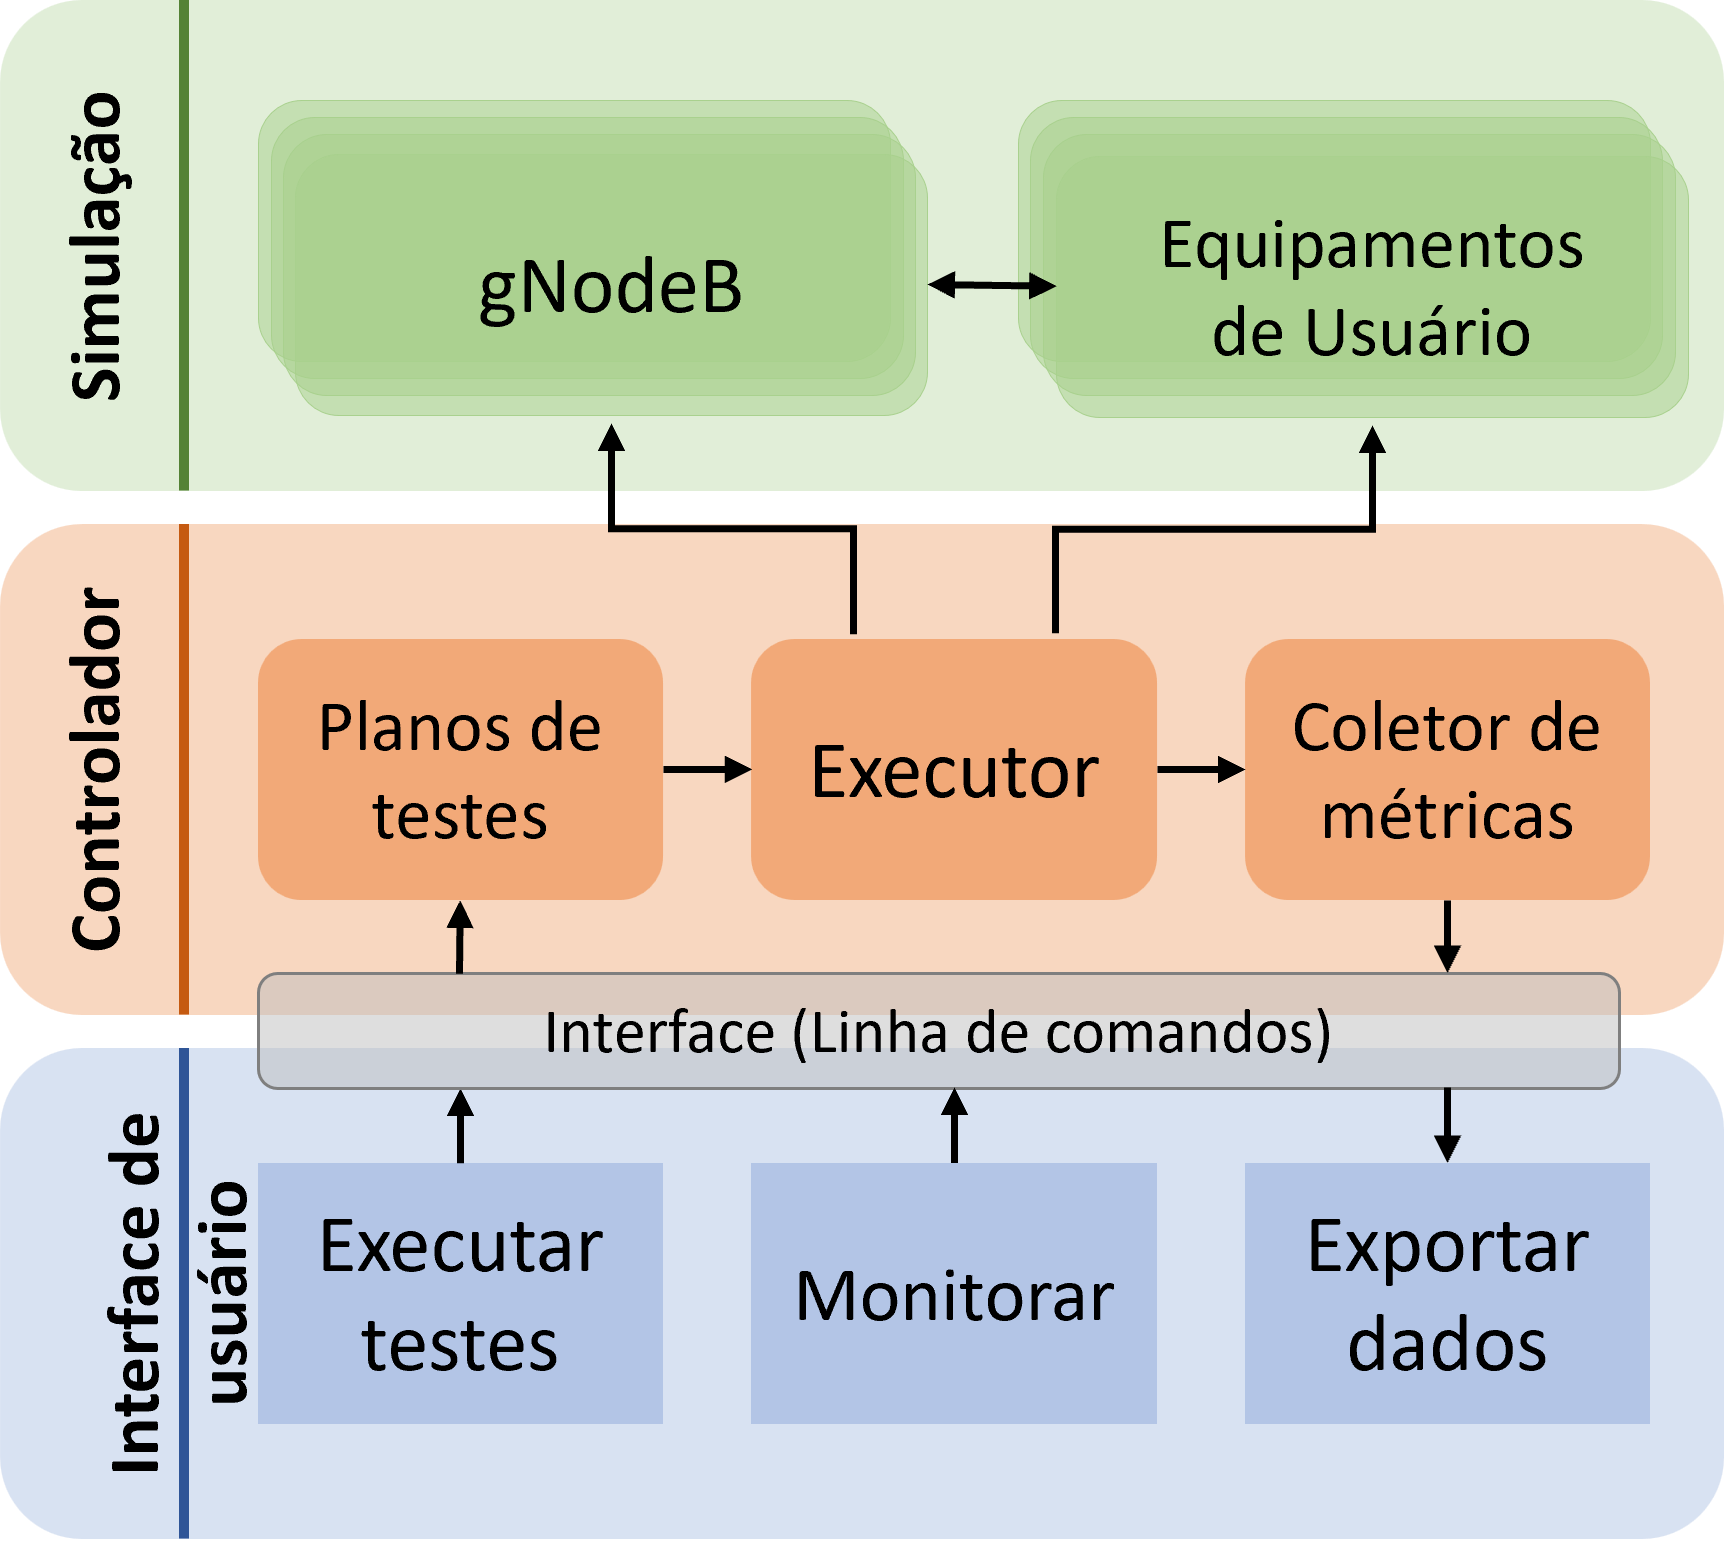
\includegraphics[width=0.6\textwidth]{TG2/Chapters/Soluction/Figures/Arquitetura-Componentes.png}
    \caption{Arquitetura do testador}
    \label{fig:tester_arch}
\end{figure}


Para desenvolver este trabalho, além do módulo implementado internamente no testador, também foi necessário desenvolver algumas ferramentas para a automação da criação e configuração do ambiente de testes e da execução dos experimentos. Essas ferramentas orquestram as múltiplas execuções dos experimentos e coletam os dados gerados para análise futura. A seguir, são apresentadas as ferramentas desenvolvidas no decorrer deste trabalho.

\subsection{Módulo de teste}

Para a execução de testes de desempenho, foi desenvolvido um módulo para o testador que permite a execução de múltiplas conexões de equipamentos de usuários simultâneas.
Esse módulo foi implementado suportando parâmetros de configuração para facilitar variações entre os testes. 
Desta forma, é possível definir o número de equipamentos de usuário a serem conectados, o atraso em milissegundos entre uma conexão e outra e o atraso em segundos para começar a execução do experimento.

No começo da execução, esse módulo simula uma gNodeB e inicia a conexão com o núcleo da rede. Após a conexão ser bem sucedida, é aguardado o tempo para iniciar a execução do experimento.
Ao iniciar o experimento, o módulo inicia um fluxo de trabalho em paralelo para criar uma nova instância de UE e realizar a conexão com o núcleo da rede.
Após iniciar o fluxo de trabalho em paralelo, o módulo aguarda o atraso entre conexões definido pelo usuário antes de iniciar o próximo fluxo, até que a quantidade de dispositivos definida seja atingida.

Durante a etapa de desenvolvimento do módulo, foi descoberta uma limitação na implementação do testador, que não consegue gerenciar mais que 255 UEs conectados simultaneamente.
Analisando o código, observa-se que a correção da limitação necessitaria de tempo e recursos não previstos na presente pesquisa.
Foi feito um contato com os desenvolvedores do testador sobre essa limitação, mas a solução para o problema não foi implementada até o presente momento.
Sendo assim, foi decidido criar múltiplas instâncias do testador, cada uma simulando uma gNodeB diferente, todas se conectando de forma simultânea na mesma instância do núcleo, cada uma simulando uma quantidade predefinida de UEs.
Desse modo, foi possível testar o comportamento de um núcleo de rede 5G com múltiplos UEs e gNodeB.

\subsection{Módulo de coleta de dados do testador}

O módulo de coleta de dados consiste em um fluxo de execução em paralelo que registra o tempo (em nanossegundos) que cada UE demorou para trocar entre cada estado da conexão com o núcleo da rede 5G.
As informações de tempo para cada estado de cada UE são escritas na saída de texto padrão do contêiner utilizado pela instância do testador.
Esse módulo foi implementado nesta presente pesquisa, visto que o testador não possuía suporte para a coleta dessa métrica até o presente momento.

Ao final da execução, uma aplicação foi desenvolvida para realizar o processamento das informações geradas através das diversas instâncias do testador, fazendo um pré processamento dos dados, ordenando eles com base no horário da inicialização do UE (em nanossegundos a partir do \textit{epoch time}\footnote{\textit{Epoch time} é uma unidade de medida de tempo contada a partir da data 1 de janeiro de 1970 às 00:00:00 UTC.}) e gerando um arquivo de texto separado por vírgulas, permitindo a fácil importação dos resultados através de programas de análise de dados.
Inicialmente, essa aplicação foi desenvolvida para coletar e processar os registros de uma única instância do testador, ordenando em ordem crescente pelo identificador do UE os dados no arquivo de saída.
Entretanto, foi necessário modificar essa aplicação para suportar múltiplas instâncias de testadores executando em paralelo e reordenar os dados do arquivo de saída, visto que a ordem de conexão dos dispositivos deixou de ser realizada em ordem crescente do identificador.

A aplicação consiste em um \textit{script} escrito na linguagem \textit{JavaScript}\footnote{https://developer.mozilla.org/pt-BR/docs/Web/JavaScript} que é executado dentro de um contêiner \textit{Docker}, evitando a instalação de um interpretador de \textit{JavaScript} diretamente na máquina que está executando os experimentos.

\subsection{Módulo de coleta de dados do núcleo}

O desenvolvimento deste módulo teve a contribuição dos bolsistas de iniciação científica do projeto PORVIR-5G.
Esse módulo consiste na implementação de um fluxo sobre uma instância da aplicação \textit{Node-RED}\footnote{https://nodered.org/}.

Um fluxo foi desenvolvido para listar todos os contêineres em execução na máquina e realizar a coleta das métricas do \textit{Docker} e armazená-las em uma instância do banco de dados \textit{InfluxDB}\footnote{https://www.influxdata.com/}. Esse fluxo foi definido para ser executado automaticamente após a inicialização do contêiner do \textit{Node-RED}, permitindo a coleta de dados de uso de disco, rede, processador, memória, entre outras, de forma automatizada pelo orquestrador do experimento.

\subsection{Orquestrador}
\label{sub:arch-orchestrator}

Com o objetivo de realizar todas as execuções dos experimentos de forma mais semelhante possível, foi desenvolvido um orquestrador que gerencia toda a execução do experimento.
O orquestrador consiste em uma série de roteiros de execução, desenvolvidos em sua maioria sobre as linguagens \textit{Bash Script} e \textit{JavaScript}.
A Figura \ref{fig:flux_orq} representa um fluxograma do algoritmo de execução do orquestrador.
O orquestrador é executado através de uma interface de usuário por linha de comandos, suportando diversos comandos para definir os parâmetros de execução do experimento, permitindo ao usuário automatizar a execução de experimentos de forma simplificada.

Os parâmetros suportados são a quantidade total de equipamentos de usuário a serem conectados no núcleo da rede, a quantidade de testadores que serão executados em paralelo, o tempo em milissegundos para ser aguardado entre cada conexão de equipamento de usuário, o tempo em segundos para aguardar a inicialização, qual núcleo da rede 5G deve ser utilizado para executar o experimento e qual experimento será executado.
Além dos parâmetros de execução do experimento, o orquestrador também permite o usuário interromper a última execução e limpar o ambiente de testes, removendo todos os contêineres e dados gerados pelo experimento, além de permitir executar o orquestrador em modo de depuração, exibindo para o usuário todos os registros de execução.

Ao iniciar a execução do orquestrador, será feita uma análise sobre o sistema operacional, verificando se a versão necessária do \textit{Kernel} do sistema está instalada.
Após realizar esta validação, o orquestrador irá verificar se todas as dependências estão corretamente instaladas e configuradas. Caso contrário, o orquestrador fará as devidas modificações automaticamente.
Uma vez que o sistema está pronto, é iniciada a execução do experimento desejado.
Primeiramente, o código-fonte do núcleo da rede 5G escolhido será baixado, compilado e seus arquivos binários serão armazenados em uma imagem de contêiner \textit{Docker}, que será iniciada na sequência.
Após a inicialização do núcleo, a base de dados desse núcleo é preenchida com as informações necessárias para a conexão dos UEs de acordo com as configurações do experimento.
Concluindo-se essa etapa, é iniciado o módulo de coleta de dados do núcleo, descrito anteriormente.
Por fim, inicia-se o contêiner do testador com os parâmetros definidos pelo usuário.

O orquestrador foi desenvolvido para suportar diferentes implementações de núcleos da rede 5G. Para isso, foi desenvolvida uma interface genérica para a inicialização do núcleo. Assim, para adicionar o suporte a um novo núcleo, basta implementar essa interface para o núcleo desejado e adicioná-la ao orquestrador.
Para a realização deste trabalho, foi desenvolvido o suporte para as implementações de núcleo 5G \textit{free5GC}, \textit{Open5GS} e \textit{OpenAirInterface}.
Todos os códigos fontes utilizados no desenvolvimento da presente pesquisa encontram-se no repositório do projeto PORVIR-5G\footnote{https://github.com/PORVIR-5G-Project} disponível através da plataforma \textit{GitHub}.

\begin{figure}[!ht]
    \centering
    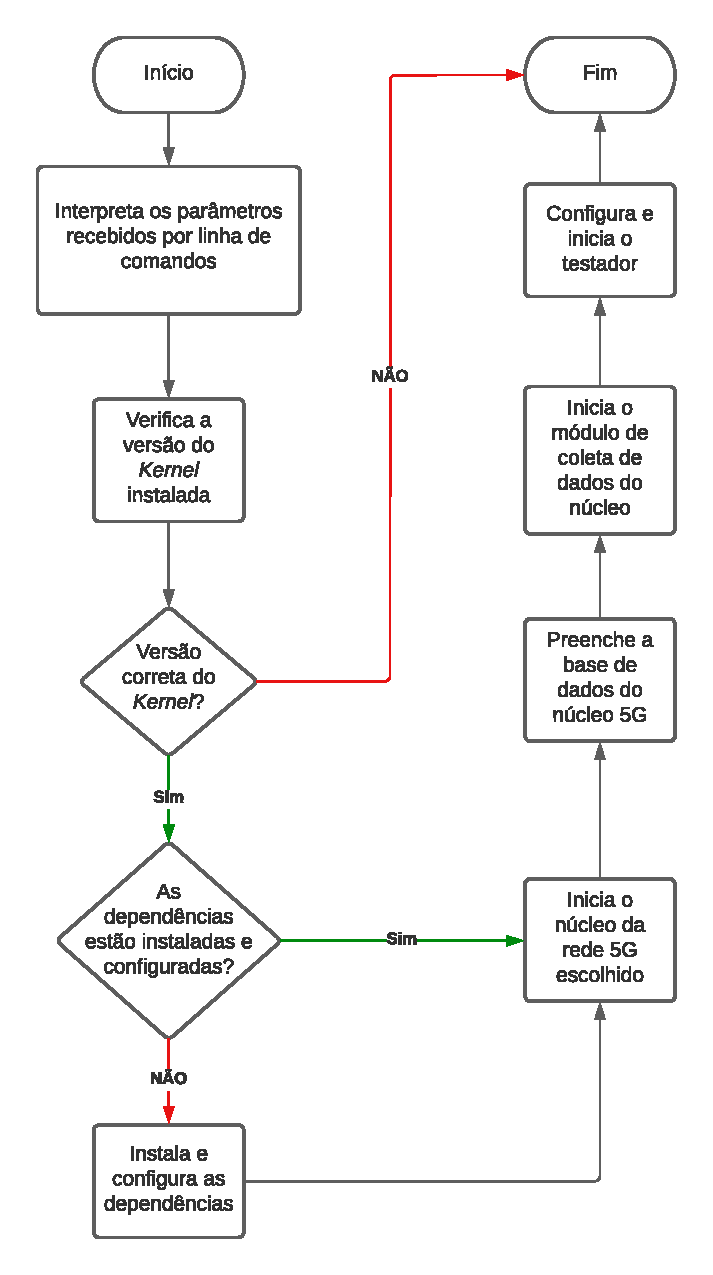
\includegraphics[width=0.55\textwidth]{TG2/Chapters/Soluction/Figures/Fluxograma-Orquestrador.pdf}
    \caption{Fluxograma de execução do orquestrador}
    \label{fig:flux_orq}
\end{figure}




\chapter{Análise dos dados coletados}
\label{chap:results}
Esse capítulo introduz a infraestrutura para realização dos testes, quais foram os experimentos realizados e as métricas utilizadas. Também apresenta os resultados dos experimentos e as conclusões geradas a partir da análise dos dados coletados.

\section{Infraestrutura e parâmetros}

Para a realização dos experimentos e validação dos resultados foi utilizada uma máquina virtual hospedada no software \textit{Kernel-based Virtual Machine} (KVM) sobre o sistema operacional \textit{TrueNAS Scale}\footnote{https://www.truenas.com/truenas-scale/}.
A máquina virtual executa o sistema operacional Ubuntu Server 20.04.4 LTS e possui diferentes configurações de processador e memória RAM, variando entre 4, 6, 8 e 12 núcleos virtuais de um processador \textit{Intel Core i7 8700T}, 4 e 8 GB de memória RAM DDR4-2666 e um disco virtual de 64 GB armazenado em um SSD M.2 NVMe.
Detalhes resumidos da máquina virtual podem ser consultados na Tabela \ref{tab:vm-config}.

Para a execução dos experimentos, foi criada uma imagem de base da máquina virtual pré-configurada, que era restaurada ao fim de cada execução do experimento, evitando que resquícios de uma execução anterior pudessem afetar outras execuções do experimento.
Além disso, também foi utilizado o sistema de conteinerização \textit{Docker}\footnote{https://www.docker.com/} para isolar os componentes do núcleo da rede 5G e do testador.

% Please add the following required packages to your document preamble:
% \usepackage{multirow}
\begin{table}[!ht]
\centering
\caption{Configuração da máquina de testes}
\label{tab:vm-config}
\begin{tabular}{|l|cccc|}
\hline
                                      & \multicolumn{4}{c|}{\textbf{Máquinas Virtuais}}    \\ \hline
\multirow{2}{*}{\textbf{CPU}}         & \multicolumn{4}{c|}{Intel Core i7 8700T @ 2.4 GHz} \\ \cline{2-5} 
 & \multicolumn{1}{c|}{4 núcleos} & \multicolumn{1}{c|}{6 núcleos} & \multicolumn{1}{c|}{8 núcleos} & 12 núcleos \\ \hline
\multirow{2}{*}{\textbf{Memória RAM}} & \multicolumn{4}{c|}{DDR4 2666 MHz}                 \\ \cline{2-5} 
 & \multicolumn{1}{c|}{4 GB}      & \multicolumn{1}{c|}{8 GB}      & \multicolumn{1}{c|}{8 GB}      & 8 GB       \\ \hline
\textbf{Armazenamento}                & \multicolumn{4}{c|}{SSD M.2 64 GB NVMe}            \\ \hline
\textbf{Sistema Operacional}          & \multicolumn{4}{c|}{Ubuntu Server 20.04.4 LTS}     \\ \hline
\end{tabular}
\end{table}

Dois experimentos distintos foram realizados sobre diferentes configurações dessa infraestrutura.
Os experimentos foram os testes de tempos de registro e estabelecimento de sessão do núcleo 5G e testes de desempenho do plano de dados do núcleo 5G.

\subsection{Testes de tempos de registro e estabelecimento de sessão do núcleo 5G}

O experimento para medição de tempos de registro e estabelecimento de sessão do núcleo 5G consiste na simulação de múltiplos UEs tentando se conectar e estabelecer uma sessão PDU com o núcleo 5G a ser testado.
Desse modo, é possível medir a latência entre cada estágio da conexão e sua variação de acordo com a carga de trabalho aplicada sobre o núcleo.
Para que fosse possível medir essa latência em diferentes cenários de forma automatizada, foi adicionado parâmetros de configuração tanto no orquestrador do experimento quanto no módulo de testes.
Neste experimento, também foram coletadas as métricas de uso de processador, memória RAM, disco e rede de todos os componentes do núcleo da rede 5G e do testador, utilizando-se as ferramentas para exportação de métricas dos contêineres \textit{Docker}.

Para esse experimento, foi utilizada a configuração da máquina virtual com 12 núcleos virtuais e 8 GB de memória RAM.
Em relação às configurações do experimento, foram utilizadas as versões dos núcleos 5G \textit{free5GC} v3.2.1, sendo a mais recente disponível no momento da execução dos experimentos e \textit{Open5GS} v2.3.6, que é a versão recomendada pelos desenvolvedores do testador.
Para cada núcleo, foram usadas as seguintes configurações do testador: número de gNB variando de 1 a 11, com passo de 2, intervalo entre conexões de 100 ms até 500 ms, com passo de 100 ms e cada gNB conectando 100 UEs.
Esse experimento foi executado 10 vezes, para obter-se uma quantidade de dados relevantes, onde ruídos externos ao experimento fossem amenizados.

Durante os testes para a realização desse experimento, algumas limitações foram encontradas e devem ser ressaltadas.
Primeiramente, pretendia-se utilizar a versão do núcleo \textit{free5GC} v3.0.6, que é recomendada pelos desenvolvedores do testador. Entretanto, essa versão do núcleo apresentou falhas após conectar aproximadamente 10 UEs, o que inviabilizaria a execução desse experimento.
O núcleo OAI apresentou uma limitação parecida tanto na versão v1.3.0, que é recomendada para o testador, quanto na versão v1.4.0, que é a mais recente disponível até o presente momento, falhando após conectar exatamente 15 UEs.
O núcleo \textit{Open5GS} na versão v2.3.6 consegue conectar exatamente 1024 dispositivos simultâneos antes de apresentar erros na função de rede AMF. Sendo assim, foi decidido que o limite de gNBs seria 11, com o total de 1100 UEs sendo conectados, atingindo a limitação desse núcleo.


\subsection{Testes de desempenho do plano de dados do núcleo 5G}

O experimento para medição do desempenho do plano de dados do núcleo 5G consiste na simulação de 1 ou mais UEs realizando o registro no núcleo da rede e iniciando um plano de dados. Após o registro ser concluído, é medida a capacidade do plano de dados utilizando-se a ferramenta \textit{iPerf}\footnote{https://iperf.fr/} versão 2.0.

Para a execução desse experimento, foi decidido utilizar a versão 2.0 da ferramenta \textit{iPerf} ao invés da versão mais recente devido a capacidade da versão 2.0 suportar múltiplas conexões de clientes em uma única instância do servidor, além de permitir exportar as métricas do experimento em um arquivo de texto separado por vírgula, facilitando o pós processamento dos dados.
Em relação à máquina virtual utilizada, foram feitos testes variando o número de núcleos virtuais de processador entre 4, 6, 8 e 12 núcleos virtuais e variando a capacidade de memória RAM entre 4 GB e 8 GB. Cada variação na quantidade de núcleos virtuais possuía uma única configuração de memória RAM. Os detalhes das máquinas virtuais estão declarados na Tabela \ref{tab:vm-config}. 
Nesse experimento, a principal métrica a ser observada é a largura de banda, em \textit{Bytes} por segundo (Bps), representando a capacidade máxima de tráfego de dados entre o UE e a rede 5G, passando pelo componente do núcleo UPF.
Nesse experimento, também foram coletadas as métricas de uso de processador, memória RAM, disco e rede de todos os componentes do núcleo da rede 5G e do testador, utilizando-se as ferramentas para exportação de métricas dos contêineres \textit{Docker}.

Em relação aos parâmetros usados para a execução do experimento, foi utilizada a configuração de 1, 2, 4, 6, 8 e 10 gNBs com 1 UE cada registrando e conectando o plano de dados antes da execução de cada teste de desempenho. Quanto aos parâmetros da ferramenta \textit{iPerf}, foi definido o tempo de execução do experimento em 60 s, reportando as métricas do teste a cada segundo.
Os núcleos de rede 5G testados foram o \textit{free5GC} v3.0.6 e o \textit{Open5GS} v2.3.6, ambas recomendadas pelo testador.
Esse experimento foi executado 16 vezes, para obter-se uma quantidade de dados relevantes, onde ruídos externos ao experimento fossem amenizados.

Algumas limitações foram observadas durante a preparação e execução desse experimento.
Visto que no experimento anterior foi utilizada a versão mais recente do núcleo \textit{free5GC}, havia a intenção de se utilizar a mesma versão para esse experimento. Porém os tutoriais para a implantação da versão v3.2.1 falharam ao estabelecer as rotas necessárias para o plano de dados, inviabilizando a conexão entre o cliente e o servidor do \textit{iPerf}. Desse modo, foi decidido utilizar uma versão anterior deste núcleo, que havia sido homologada pelos desenvolvedores do testador.
Nesse experimento, o OAI apresentou o mesmo problema, com falhas ao estabelecer as rotas entre o UE e a rede 5G nas versões v1.3.0 e v1.4.0, sendo esta a mais recente ate o presente momento. Dessa forma, foi decidido não realizar os experimentos sobre esse núcleo.


\section{Análise e discussão dos tempos de registro e estabelecimento de sessão do núcleo 5G}
Para o experimento de medição do tempo de conexão de equipamentos de usuário, foi levado em consideração o tempo total entre o início do processo de registro e a obtenção do plano de dados. Após a coleta e processamento dos dados desse experimento, os gráficos da Figura \ref{fig:exp1_conn} foram gerados para permitir a visualização e análise dos dados coletados.
O gráfico representa o tempo médio de conexão para cada rajada de conexões simultâneas, com o eixo X representando o tempo de execução do experimento, em segundos, e o eixo Y representando o tempo total para estabelecer a conexão e iniciar o plano de dados deste equipamento de usuário, em milissegundos.
Na coluna da esquerda, são apresentados os resultados para o núcleo 5G \textit{free5GC} e, na direita, o \textit{Open5GS}. Para cada núcleo, foram desenhados 5 gráficos, com as diferentes variações de intervalo entre rajadas de conexões de UEs.

Ao analisar os dados, é possível inferir que, para as condições do experimento, o núcleo \textit{free5GC} possuiu tempo de conexão médio de 1089 ms, quando cada conexão se iniciou 500 ms após a anterior.
Nesse experimento, a mediana do tempo de conexão foi de 853 ms e o tempo máximo de conexão foi de 5,57 segundos.
Para um intervalo entre conexões de 100 ms, o tempo médio de conexão foi de 7731 ms, tendo sua mediana em 3027 ms e o tempo máximo de conexão durando pouco mais de 54 segundos.

Quanto ao comportamento do núcleo de rede 5G \textit{Open5GS}, percebe-se que para um intervalo de 500 ms, o tempo médio foi de 306 ms, com sua mediana em 305 ms e seu tempo máximo de conexão em 345 ms.
Para o intervalo de 100 ms, a média subiu para 364 ms, enquanto a mediana subiu para 358 ms e o valor máximo atingiu 490 ms.
Desse modo, considerando-se apenas o tempo de conexão, o núcleo de rede \textit{Open5GS} possui melhor desempenho, aguentando diversas rajadas de conexões em diferentes cenários, tendo seu tempo médio variando em torno de 58 milissegundos. O núcleo \textit{free5GC} possui uma variação de aproximadamente 49 segundos entre as diferentes execuções do experimento.
Os dados detalhados para cada execução desse experimento podem ser vistos na Tabela \textcolor{red}{INSERIR TABELA}.

\begin{figure}[H]
    \centering
    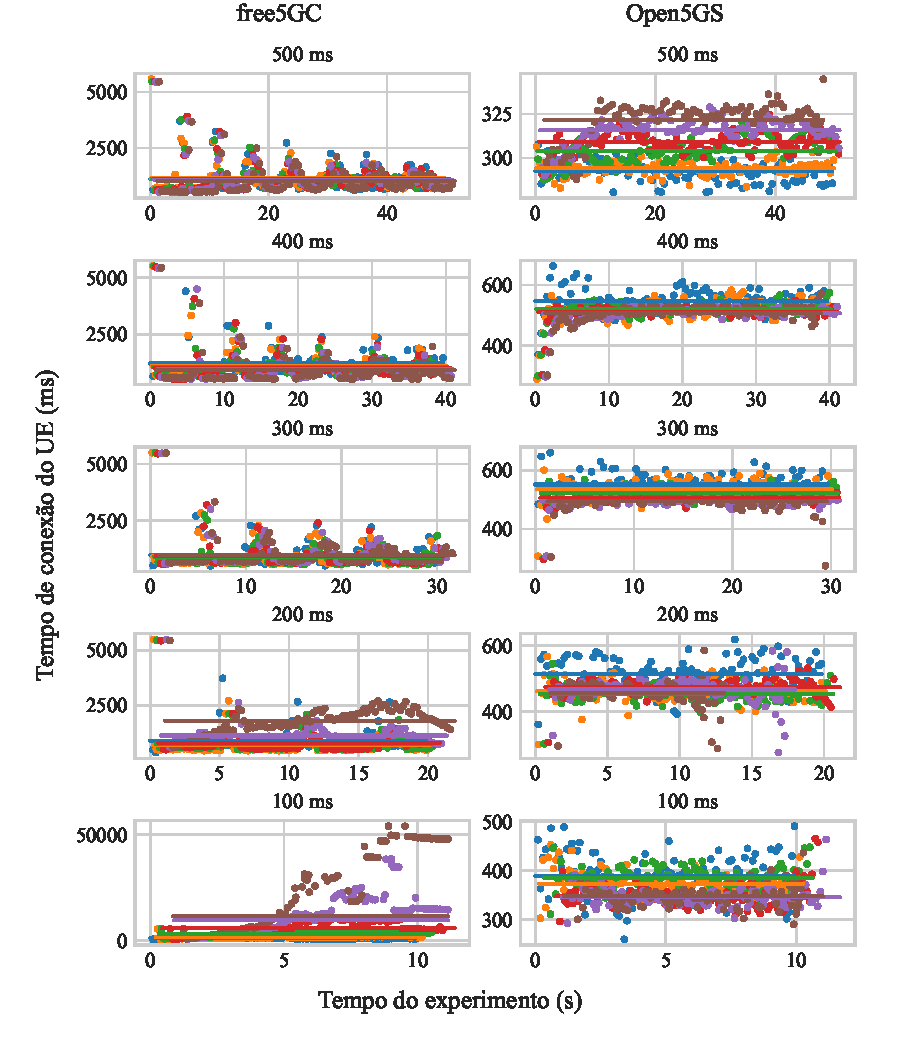
\includegraphics[width=0.85\textwidth]{TG2/Chapters/DataAnalysis/Figures/EXP1-CONN-12C-8GB.pdf}
    \caption{Tempo de registro e estabelecimento de sessão PDU para cada núcleu 5G}
    \label{fig:exp1_conn}
\end{figure}

Durante a execução dos experimentos, a taxa de conexões mal sucedidas entre o UE e o núcleo da rede foi significativa entre cada execução do experimento para cada um dos núcleos testados. Sendo assim, foi desenhado os gráficos da Figura \ref{fig:exp1_conn_err} com a comparação de taxa de erro média entre os dois núcleos avaliados.
Cada gráfico representa a taxa de erro média de conexão dos UEs com os núcleos testados, com o intervalo de tempo entre as rajadas em ordem decrescente, de 500 a 100 ms, com passos de 100 ms.
As barras dos gráficos representam a média de erros entre as execuções do experimento realizadas para cada configuração de gNB e núcleo, enquanto as linhas representam o desvio padrão da média para cada execução do experimento.

Nesse experimento, foi possivel observar que o núcleo \textit{free5GC} possui uma taxa de erros de conexão crescente para cada gNB adicionada. Ao adicionar uma gNB, a taxa de conexões simultâneas aumentava na mesma proporção que a taxa de erros.
Esse comportamento pode ser percebido no núcleo \textit{Open5GS} quando se reduz o intervalo entre rajadas de conexões para um valor menor que o tempo médio necessário para se estabelecer a conexão.
Entretanto, para intervalos maiores de tempo, o núcleo \textit{Open5GS} apresentou boa estabilidade no geral, tendo em alguns momentos a taxa de erros de conexão igual a zero.

Através da análise desses resultados, percebe-se que o núcleo de rede 5G \textit{Open5GS} possui maior estabilidade para o registro de sessões dos UE em escala em comparação com o núcleo \textit{free5GC}.
Apesar desses resultados, foi descoberta uma limitação no núcleo \textit{Open5GS} em relação à quantidade máxima de dispositivos conectados simultaneamente, sendo essa igual a 1024 dispositivos.
É importante ressaltar que essa limitação não está presente no núcleo \textit{free5GC}.
Os dados detalhados para cada execução desse experimento podem ser vistos na Tabela \textcolor{red}{INSERIR TABELA - TALVEZ SEJA A MESMA DE CIMA}.

\begin{figure}[H]
    \centering
    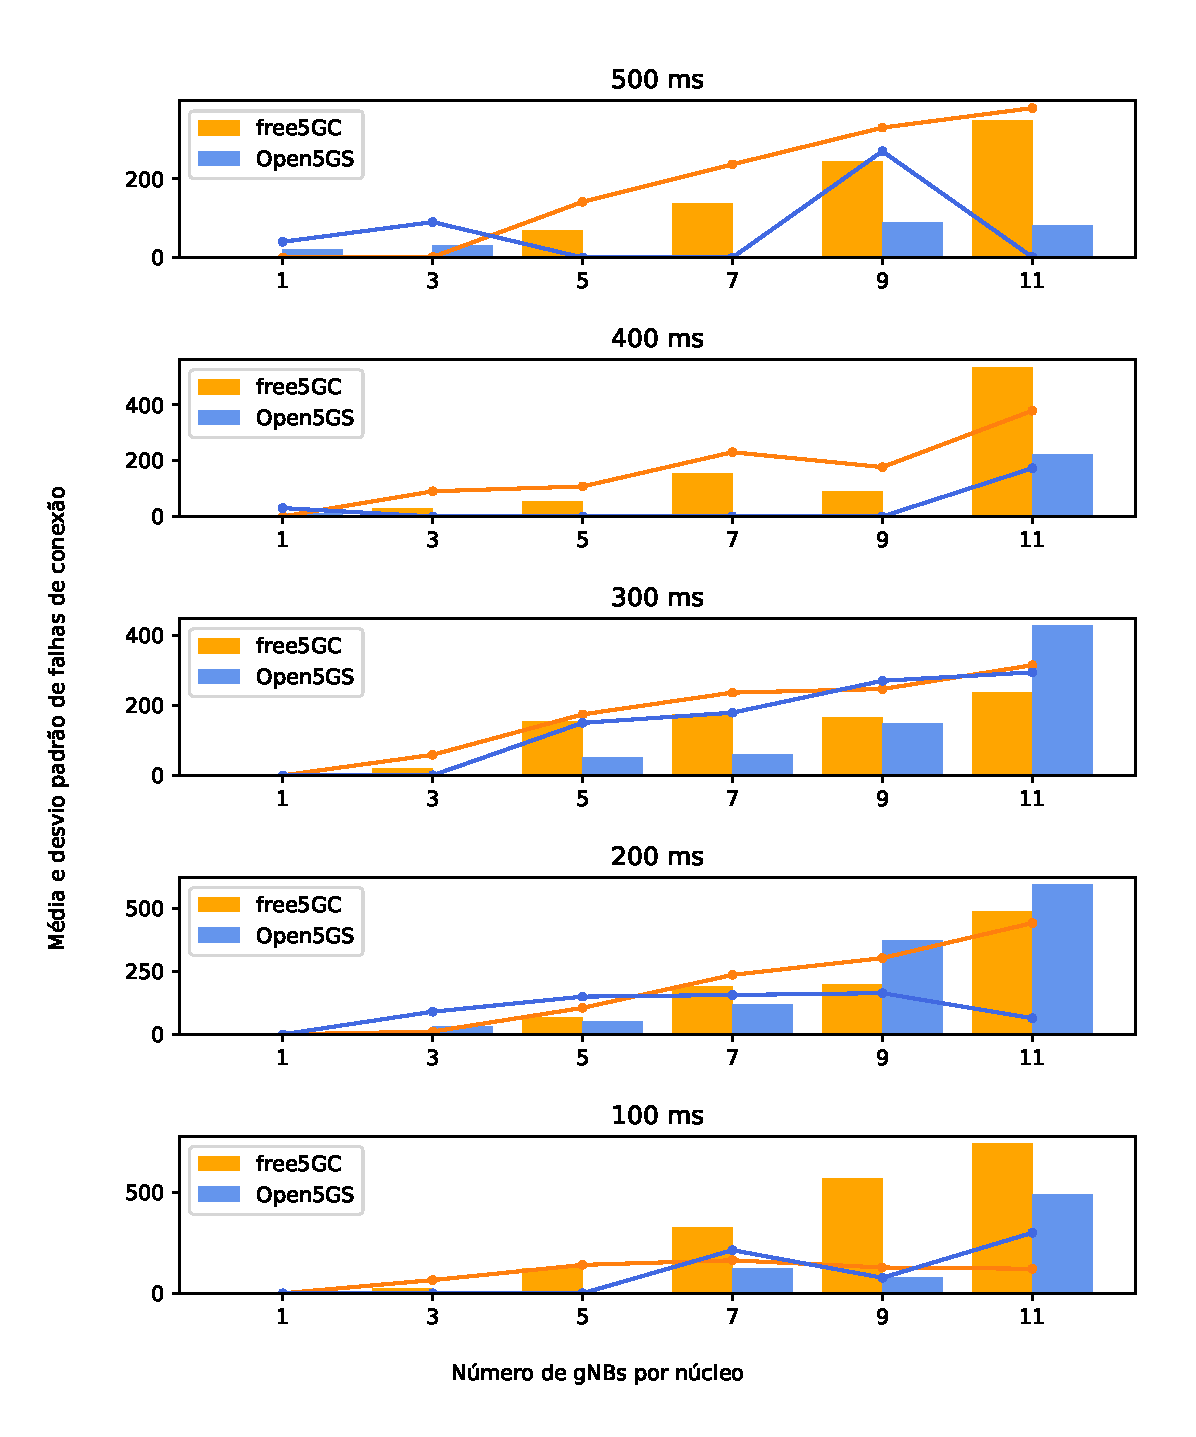
\includegraphics[width=0.95\textwidth]{TG2/Chapters/DataAnalysis/Figures/EXP1-CONN_ERR-12C-8GB.pdf}
    \caption{Média e desvio padrão dos erros de conectividade nos experimentos executados}
    \label{fig:exp1_conn_err}
\end{figure}


\section{Análise e discussão dos resultados em relação ao desempenho do plano de dados}
Para o experimento de avaliação do desempenho do plano de dados do núcleo da rede 5G, foi executada, por 60 segundos, a ferramenta \textit{iPerf} 2.0 simultaneamente em cada UE conectado ao núcleo 5G.
Em um primeiro momento, foi utilizada a máquina virtual em sua configuração máxima, com 12 núcleos virtuais de CPU e 8 GB de memória RAM.
Após a coleta e o processamento dos dados gerados pela ferramenta \textit{iPerf}, foram gerados os gráficos representando a largura de banda por segundo dos núcleos de rede 5G \textit{free5GC} e \textit{Open5GS} testados.

A Figura \ref{fig:exp2_free5gc_12-8} apresenta os gráficos com a largura de banda para cada configuração de quantidade de UE para o núcleo \textit{free5GC} na máquina virtual com 12 núcleos virtual de processador e 8 GB de memória RAM.

\begin{figure}[H]
    \centering
    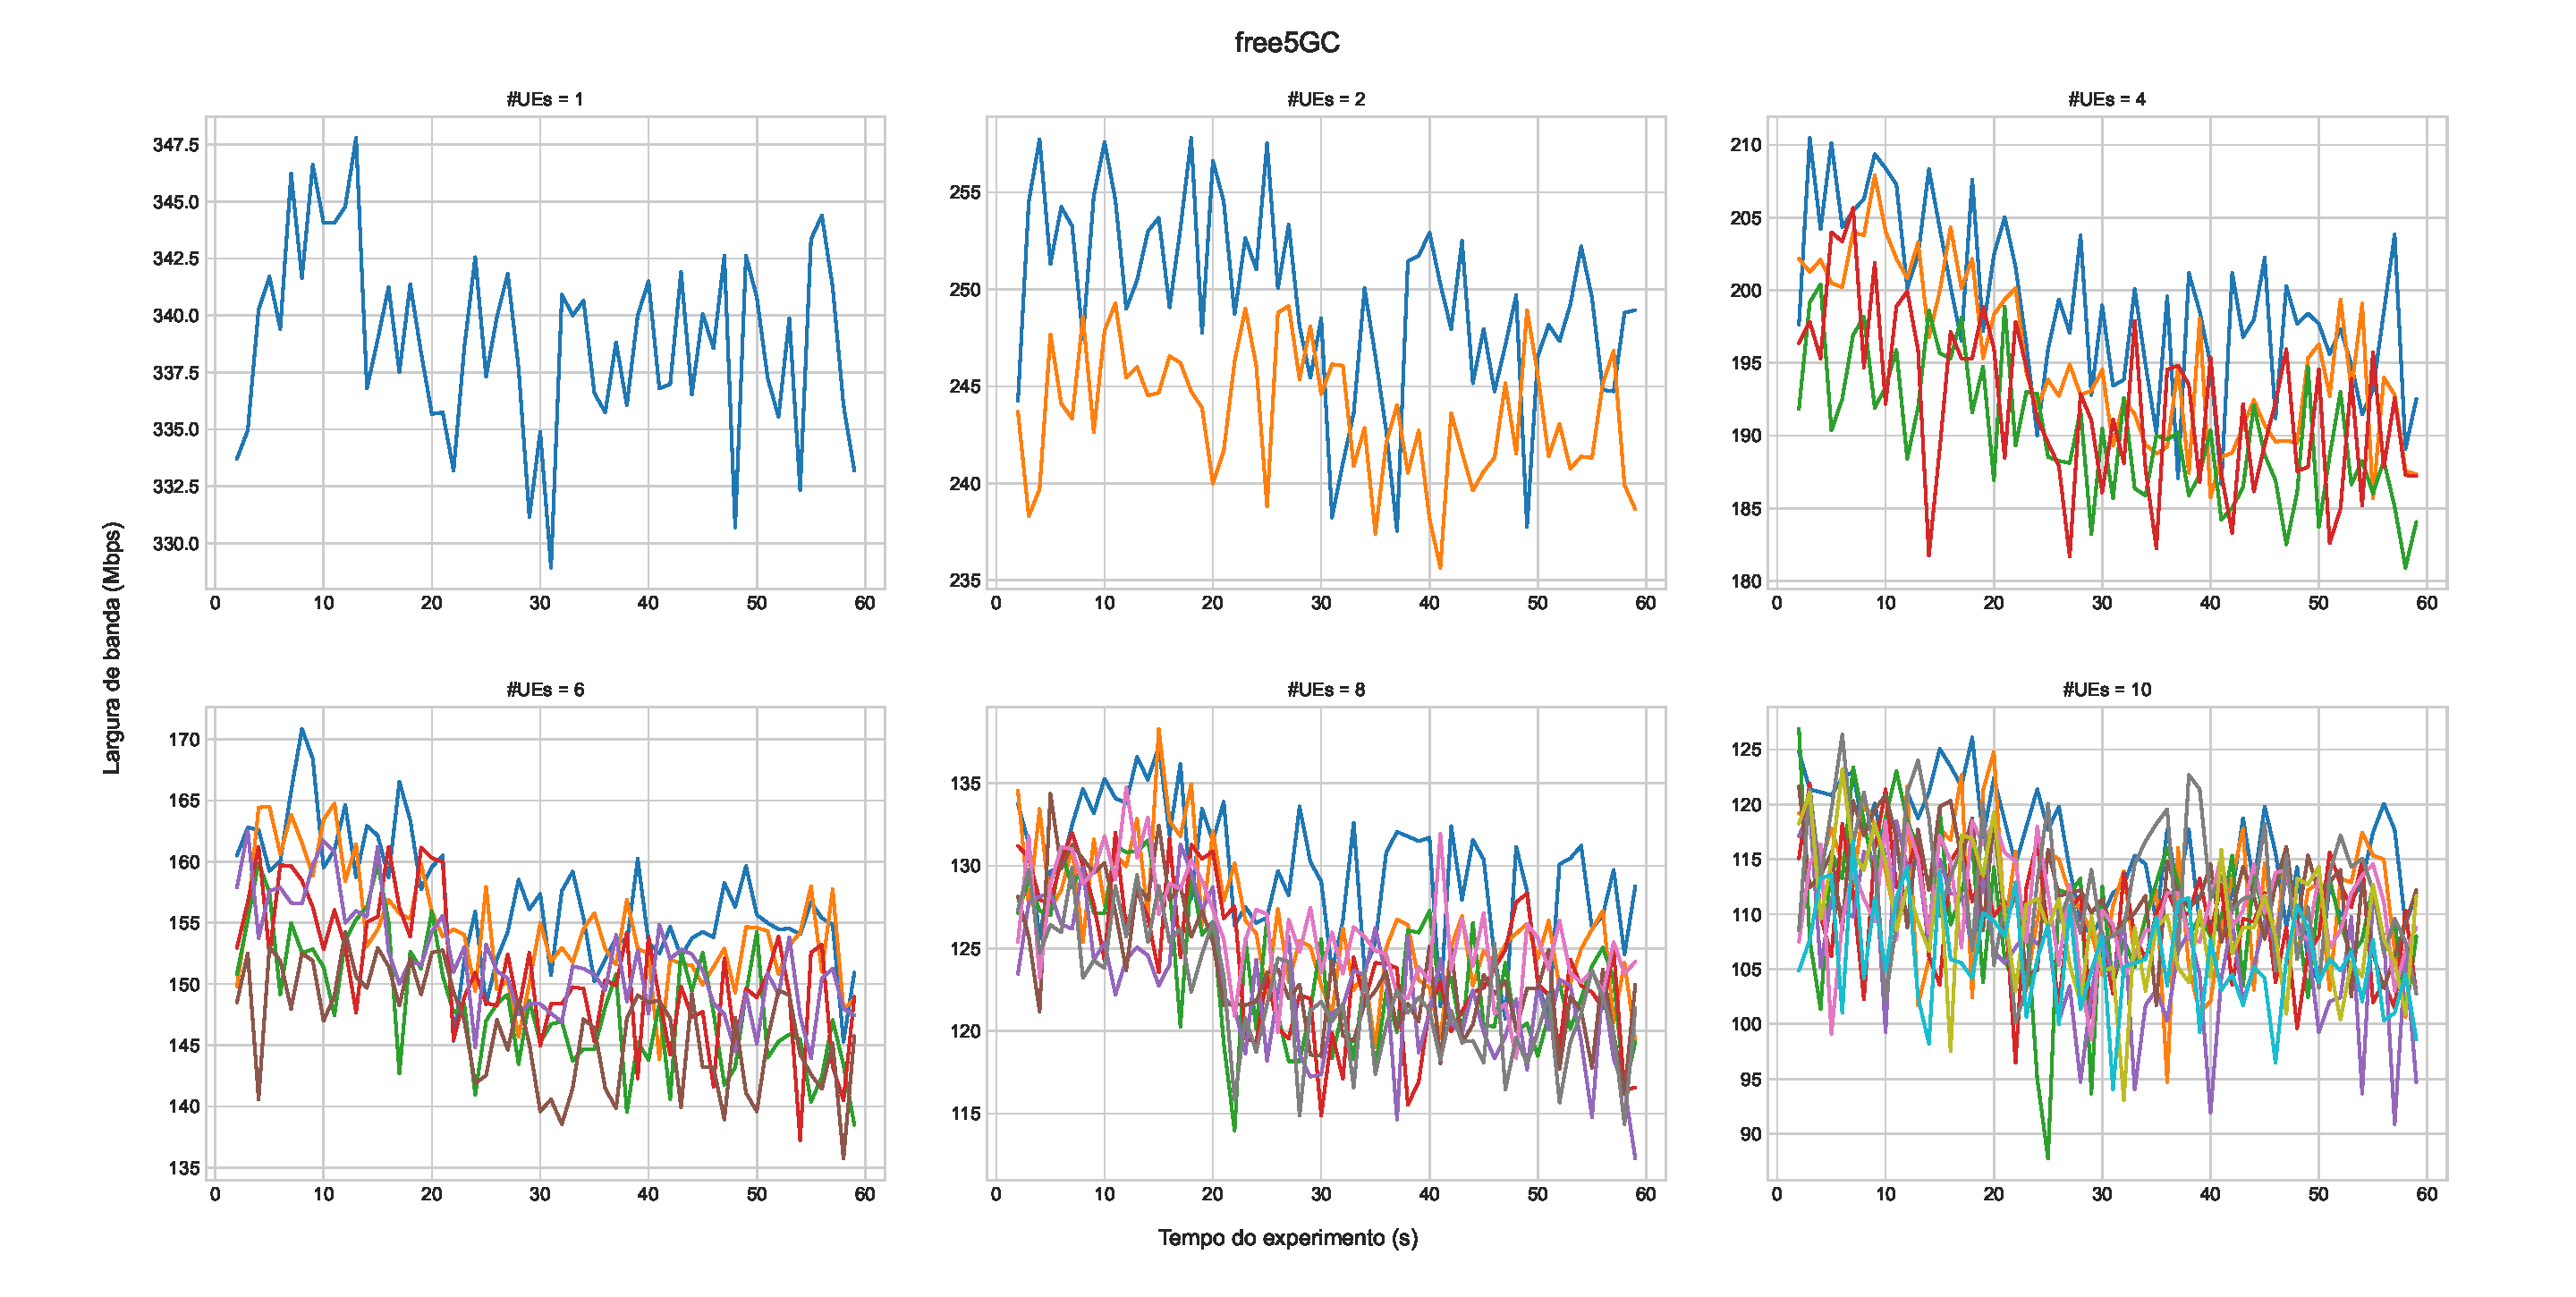
\includegraphics[width=1\textwidth]{TG2/Chapters/DataAnalysis/Figures/EXP2-free5GC-12C-8GB.pdf}
    \caption{Largura de banda para cada configuração de quantidade de UE para o núcleo \textit{free5GC}}
    \label{fig:exp2_free5gc_12-8}
\end{figure}

A Figura \ref{fig:exp2_open5gs_12-8} apresenta os gráficos com a largura de banda para cada configuração de quantidade de UE para o núcleo \textit{Open5GS} na máquina virtual com 12 núcleos virtual de processador e 8 GB de memória RAM.

\begin{figure}[H]
    \centering
    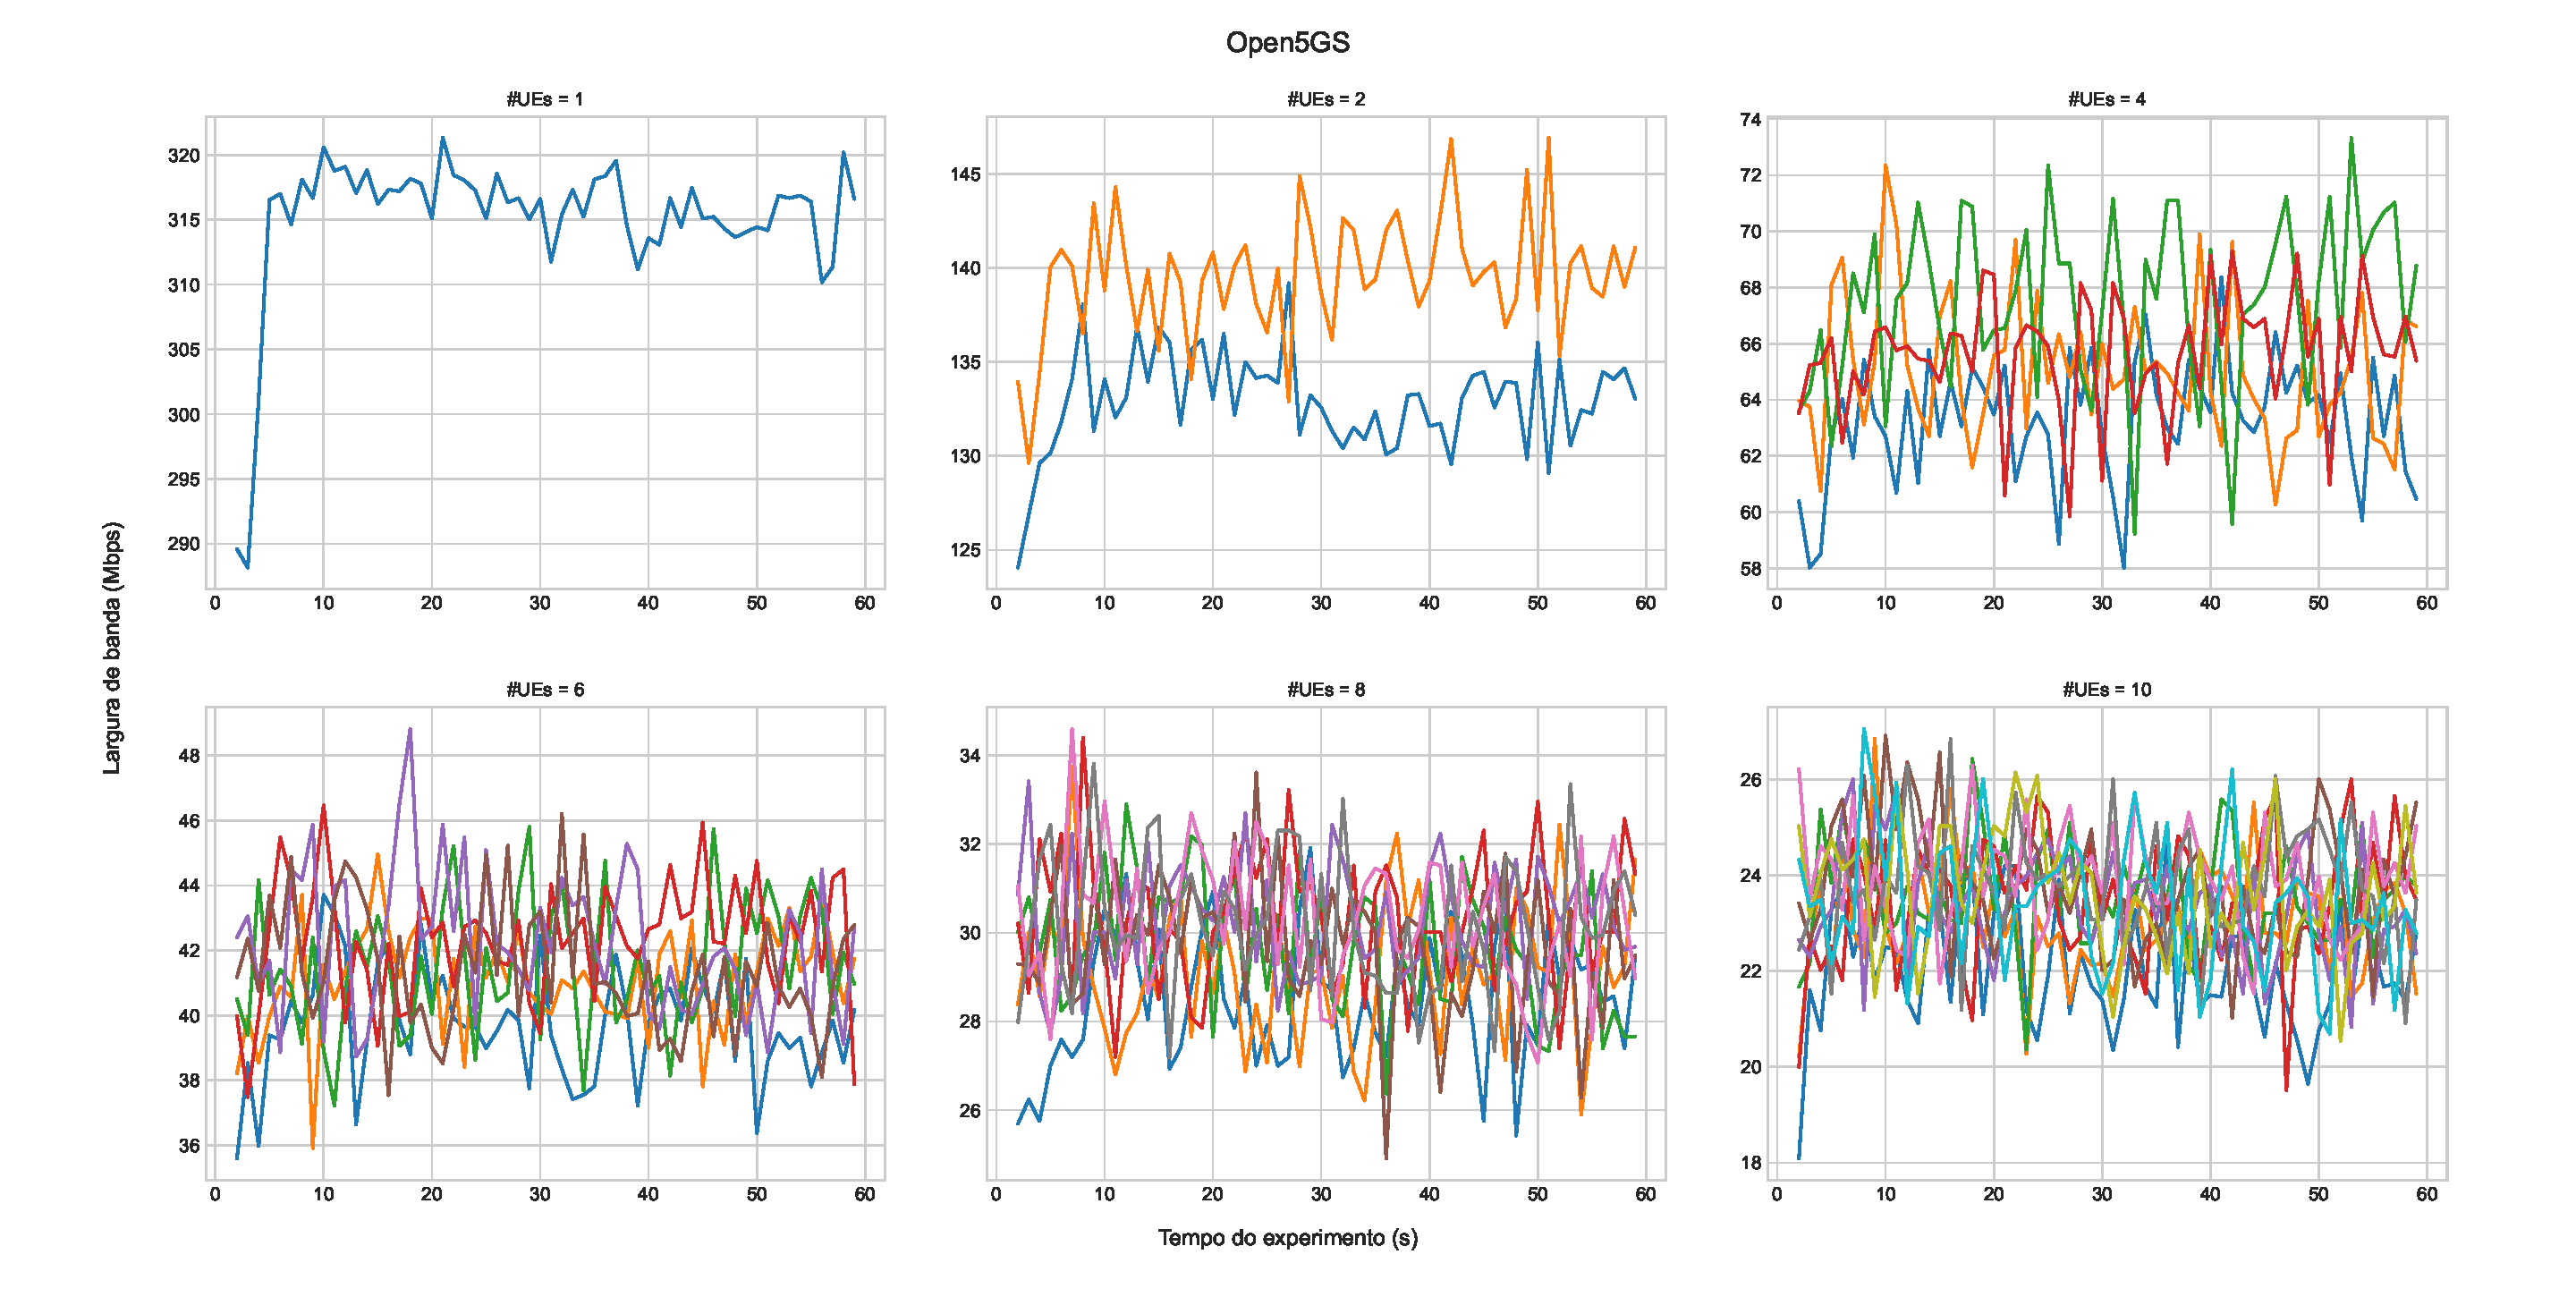
\includegraphics[width=1\textwidth]{TG2/Chapters/DataAnalysis/Figures/EXP2-Open5GS-12C-8GB.pdf}
    \caption{Largura de banda para cada configuração de quantidade de UE para o núcleo \textit{Open5GS}}
    \label{fig:exp2_open5gs_12-8}
\end{figure}

Através desses gráficos, é possível observar que a largura de banda disponível para os UEs não é estável, oscilando durante toda a execução do experimento.
Para uma melhor visualização dos valores agregados de cada execução desse experimento, foram criados gráficos de barra.
O eixo X do gráfico representa o número de UEs em cada rodada do experimento, onde segmento da barra representa o UE de mesma cor das duas figuras anteriores.
Cada barra do gráfico representa a largura de banda média em Mbps agregada entre os UEs.
A Figura \ref{fig:exp2_all_12-8} apresenta o valor agregado da largura de banda para cada configuração de quantidade de UE para a máquina virtual com 12 núcleos virtuais e 8 GB de memória RAM.

\begin{figure}[H]
    \centering
    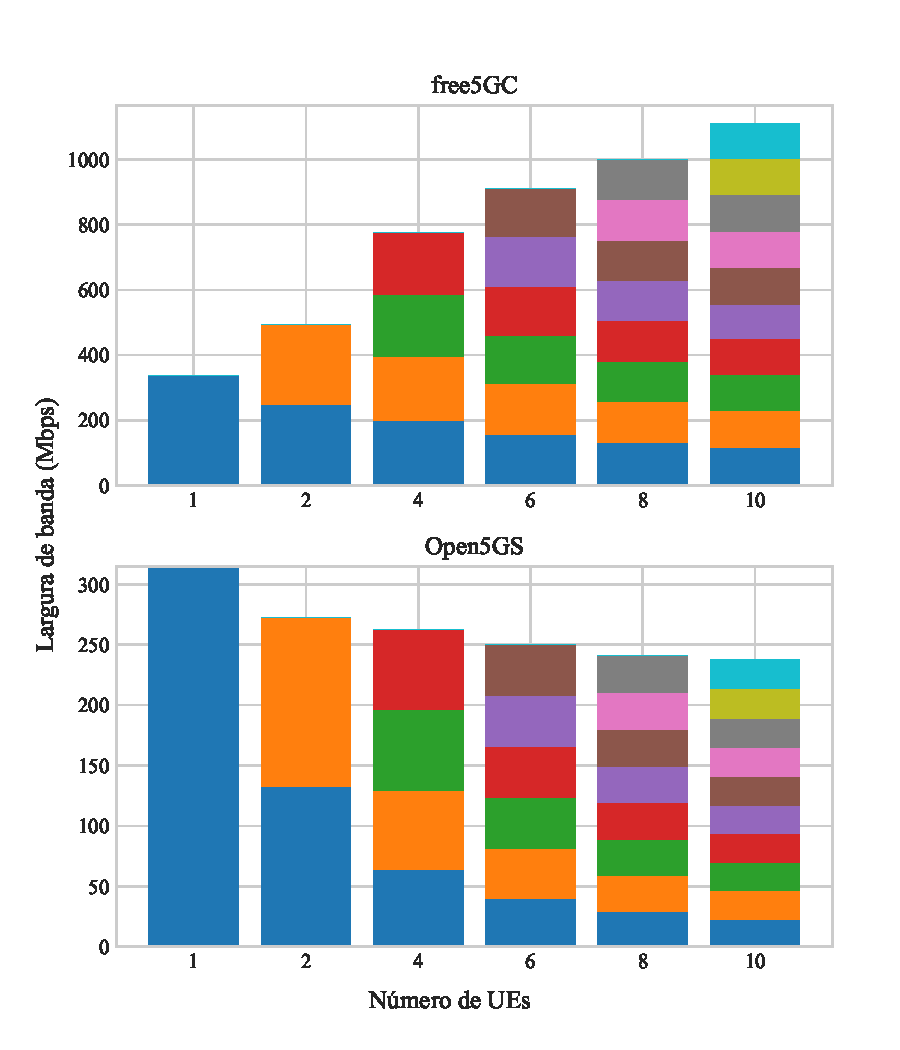
\includegraphics[width=1\textwidth]{TG2/Chapters/DataAnalysis/Figures/EXP2-ALL-12C-8GB.pdf}
    \caption{Valor agregado da largura de banda para cada configuração de quantidade de UEs}
    \label{fig:exp2_all_12-8}
\end{figure}

Nesse experimento, percebe-se que no núcleo \textit{free5GC} a largura de banda total entre cada execução aumenta de acordo com a quantidade de UEs conectados.
O valor médio de largura de banda para esse núcleo com um UE conectado é de 338.4 Mbps, aumentando para 777.0 Mbps com quatro UEs conectadas e 1109.9 Mbps com 10 UEs conectadas.
Em contrapartida, o comportamento do núcleo \textit{Open5GS} se opõe ao \textit{free5GC}. No núcleo \textit{Open5GS}, o valor médio da largura de banda para um UE conectado é de 314.5 Mbps, reduzindo para 262.7 Mbps com 4 UEs conectadas e 237.9 Mbps ao conectar 10 UEs simultâneas.
Esse experimento demonstra que o núcleo \textit{free5GC} possui melhor estrutura para gerenciar o tráfego de dados de UEs em escala em relação ao núcleo \textit{Open5GS}.

Ao limitar a quantidade de recursos disponíveis para a execução do experimento, diminuindo a quantidade de núcleos virtuais de processador e memória RAM da máquina virtual, percebe-se que o desempenho do plano de dados para o núcleo \textit{free5GC} é diretamente proporcional à quantidade de núcleos virtuais disponíveis.
A Figura \ref{fig:exp2_all_8-8} representa o desempenho médio agregado do plano de dados para a execução do experimento em uma máquina virtual com 8 núcleos virtuais de processador e 8 GB de memória RAM.
Nesse caso, largura de banda máxima do plano de dados para o núcleo \textit{free5GC} é reduzida para 1004.2 Mbps quando executado com dez UEs simultâneos.
Essa redução de desempenho pode ser explicada devido à limitação na carga máxima de processamento suportada pela máquina virtual.

\begin{figure}[H]
    \centering
    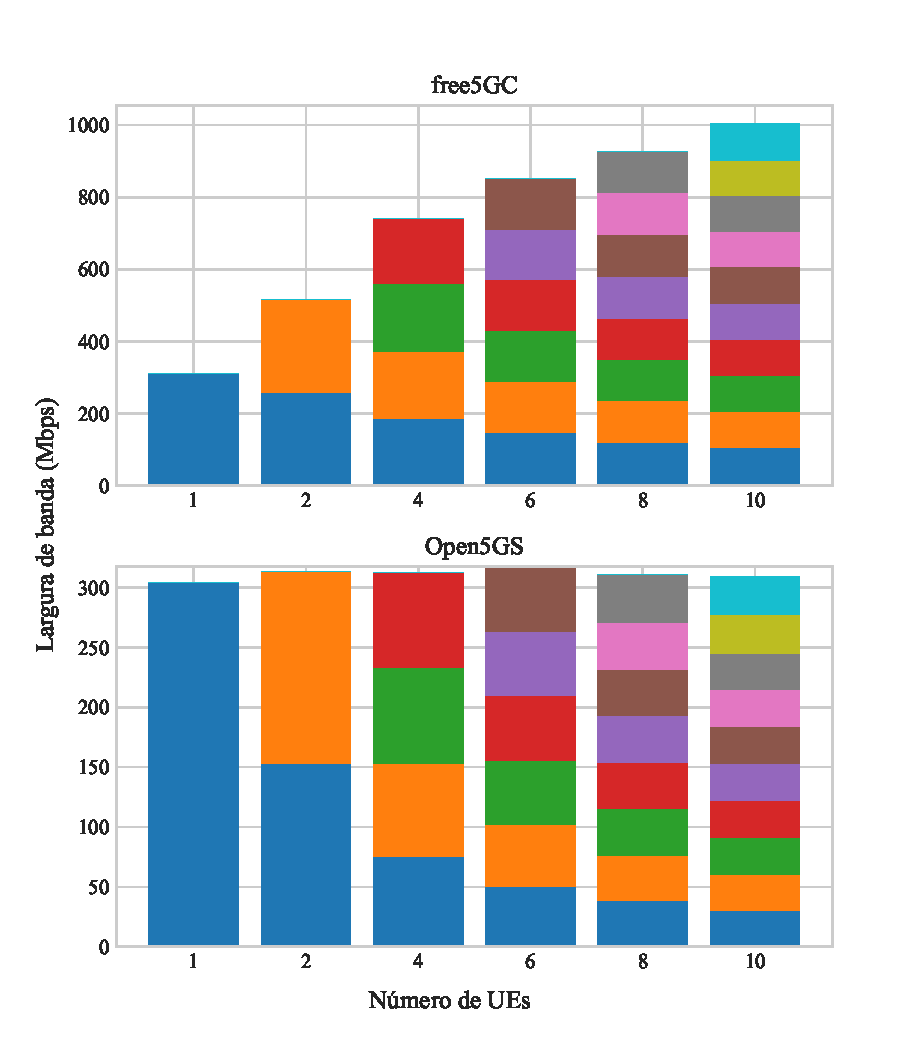
\includegraphics[width=1\textwidth]{TG2/Chapters/DataAnalysis/Figures/EXP2-ALL-8C-8GB.pdf}
    \caption{Valor agregado da largura de banda para cada configuração de quantidade de UEs}
    \label{fig:exp2_all_8-8}
\end{figure}

A redução de desempenho do plano de dados fica mais visível ao limitar-se ainda mais a quantidade de núcleos virtuais disponíveis para o experimento.
Na Figura \ref{fig:exp2_all_6-8}, onde a máquina virtual é executada com 6 núcleos virtuais de processador e 8 GB de memória RAM, é possível perceber que o desempenho máximo do plano de dados do núcleo \textit{free5GC} é atingido com seis UEs simultâneos.

\begin{figure}[H]
    \centering
    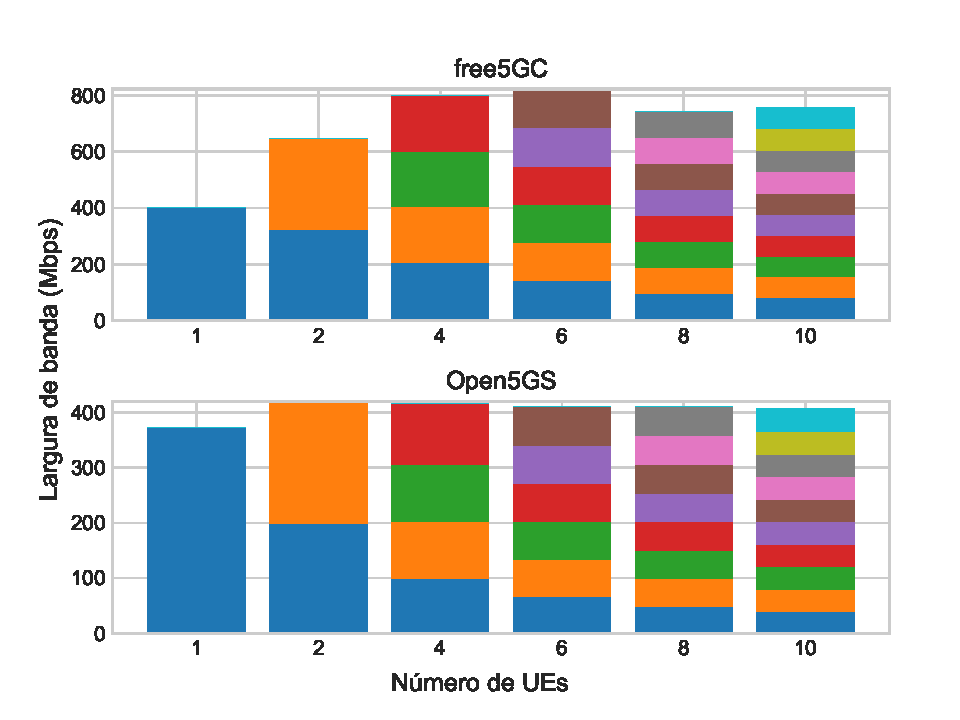
\includegraphics[width=1\textwidth]{TG2/Chapters/DataAnalysis/Figures/EXP2-ALL-6C-8GB.pdf}
    \caption{Valor agregado da largura de banda para cada configuração de quantidade de UEs}
    \label{fig:exp2_all_6-8}
\end{figure}

A Figura \ref{fig:exp2_all_4-4} representa os resultados obtidos para a execução do experimento em uma máquina virtual com 4 núcleos virtuais de processador e 4 GB de memória RAM.
Essa configuração foi utilizada para simular um cenário com recursos limitados.
Neste caso, o desempenho máximo do núcleo \textit{free5GC} ocorre com quatro UEs simultâneos. 
A redução de desempenho para testes com maior quantidade de UEs simultâneos é explicada pela sobrecarga de uso de processador causada pela quantidade de UEs trafegando dados em paralelo.

\begin{figure}[H]
    \centering
    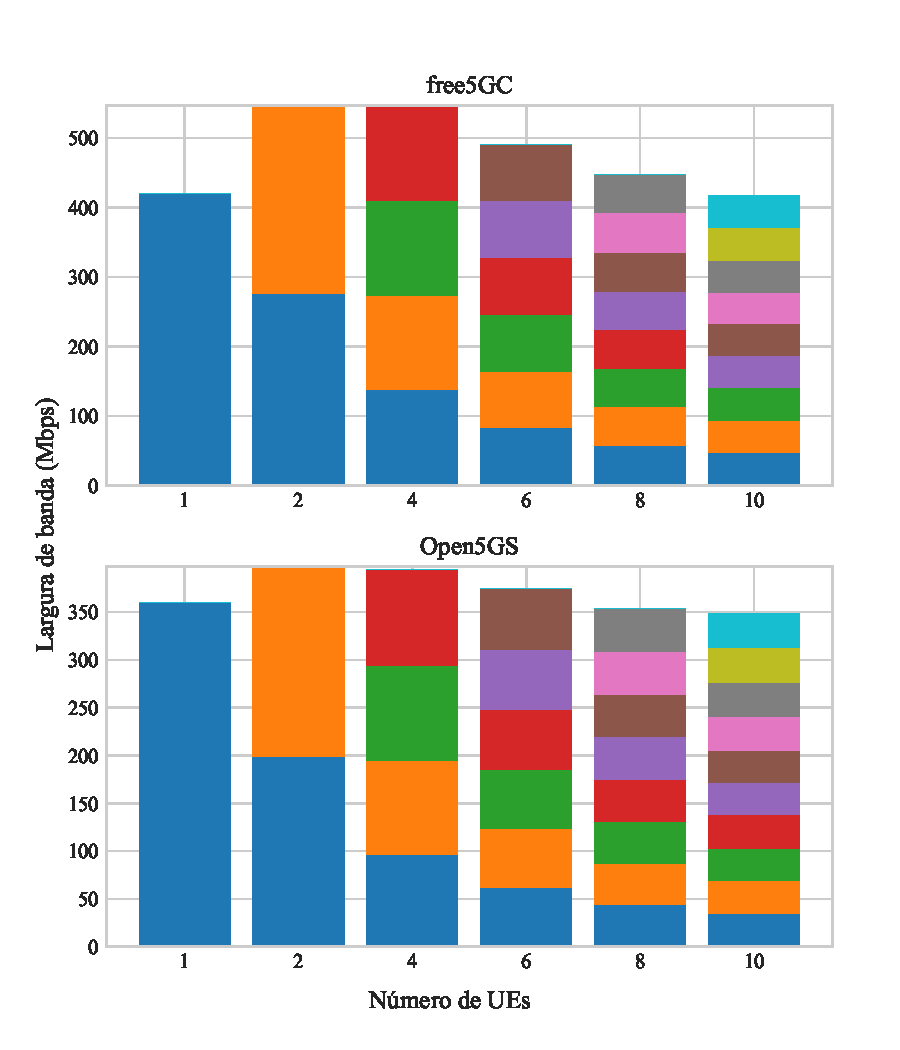
\includegraphics[width=1\textwidth]{TG2/Chapters/DataAnalysis/Figures/EXP2-ALL-4C-4GB.pdf}
    \caption{Valor agregado da largura de banda para cada configuração de quantidade de UEs}
    \label{fig:exp2_all_4-4}
\end{figure}


% \section{Análise e discussão em relação ao consumo de recursos}
% Esta seção apresenta a análise de dados de uso de processador e memória RAM da máquina virtual para a execução dos experimentos.
Os dados para cada contêiner foram agrupados em três conjuntos, para facilitar a visualização dos dados.
O primeiro conjunto representa os dados agregados de todas as instâncias do testador, denominado nos gráficos como Testadores.
O segundo conjunto representa os dados agregados de todas as funções do núcleo em teste, denominado nos gráficos como Núcleo.
O terceiro conjunto representa os dados agregados do restante dos serviços em execução, como os contêineres utilizados para rodar o módulo de coleta de dados do núcleo e o servidor da aplicação \textit{iPerf} utilizada no segundo experimento, denominado nos gráficos como Outros.
Uma análise com maiores detalhes do uso de recursos para cada componente em execução durante o período do experimento é possível ao utilizar a ferramenta para gerar visualizações dos dados coletados disponível através da aplicação \textit{InfluxDB}.
Essa ferramenta faz parte do módulo de coleta de dados do núcleo da rede.

\subsection{Análise e discussão em relação ao consumo de recursos do experimento de registro e estabelecimento de sessão do núcleo 5G}

Para a análise do uso de recursos de processador e memória RAM para a execução do experimento de registro e estabelecimento de sessão do núcleo 5G, foi utilizada uma execução do experimento com intervalo entre conexões de UEs de 500 ms sobre a máquina virtual com 12 núcleos de processador virtuais e 8 GB de memória RAM.
Os resultados agregados podem ser vistos na Figura \ref{fig:exp1_500ms_res}.

\begin{figure}[H]
    \centering
    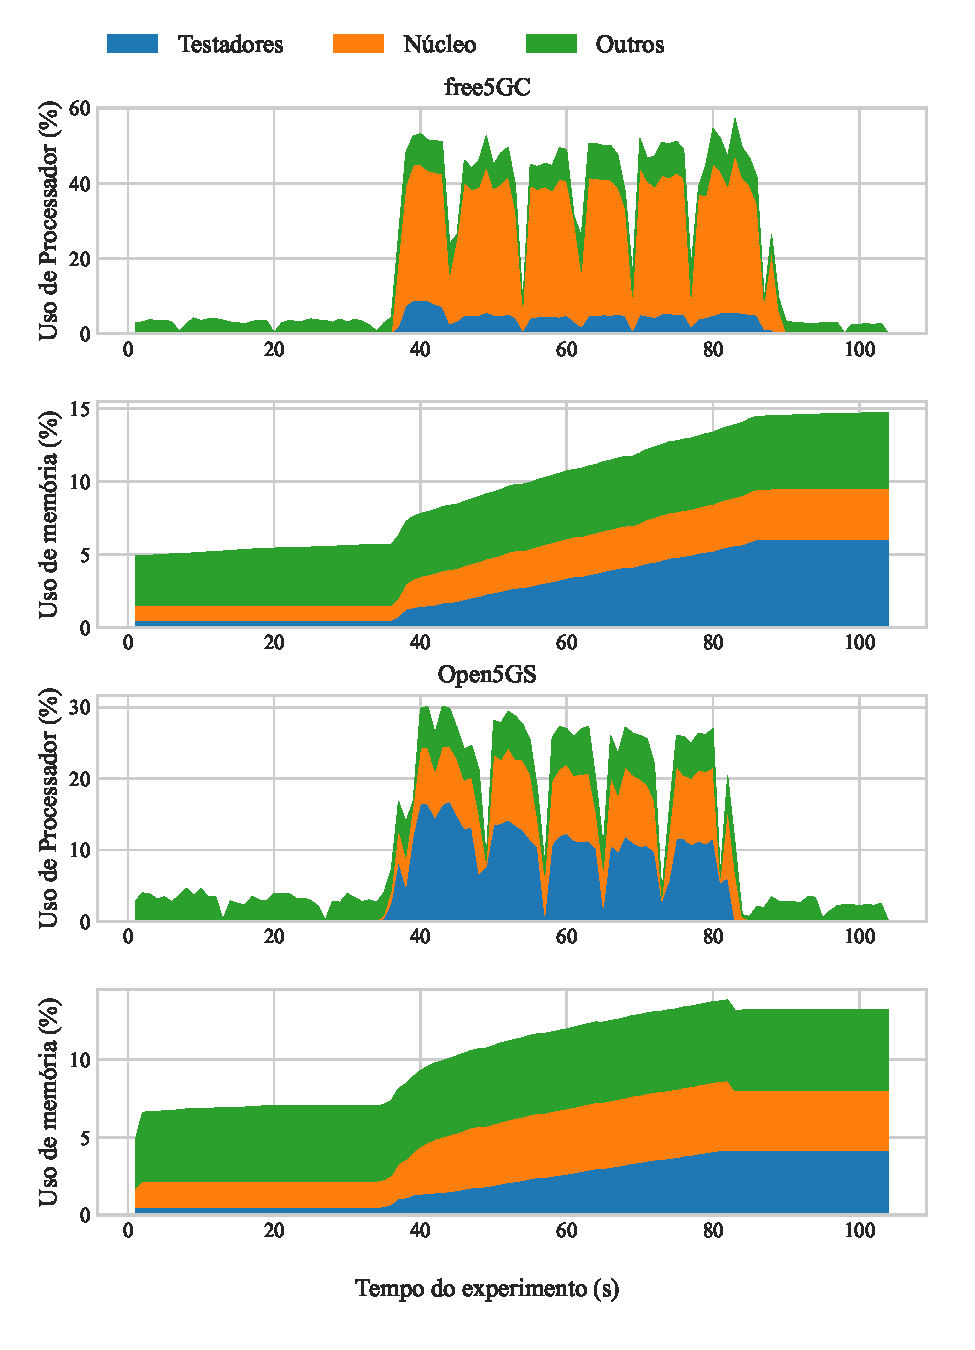
\includegraphics[width=0.95\textwidth]{TG2/Chapters/DataAnalysis/Figures/EXP1-CONN-RES-500ms-12C-8GB.pdf}
    \caption{Uso de processador e memória RAM para a execução com atraso de 500 ms entre conexões}
    \label{fig:exp1_500ms_res}
\end{figure}

Esta figura apresenta o uso de processador e memória RAM de acordo com o tempo de execução do experimento para os núcleos \textit{free5GC} e \textit{Open5GS}.
O eixo X dos gráficos representam o tempo em segundos referente à coleta de dados total do experimento, considerando o tempo para a inicialização, execução e encerramento do experimento.
O eixo Y representa a porcentagem do uso para cada tipo de recurso analisado.
As áreas azuis, laranjas e verdes dos gráficos representam a porcentagem de uso agregado de recursos para a execução dos testadores, núcleos 5G e os demais componentes, respectivamente.

Ao observar o uso de recursos somente durante o período da execução do experimento, a média de uso de processador para o núcleo \textit{free5GC} foi de 31,33\% e para o núcleo \textit{Open5GS} foi de 7,26\%.
Em relação ao uso de memória RAM, o pico de uso de memória para o núcleo \textit{free5GC} foi de 3.45\%, representando o uso de 282,6 MB de memória RAM.
Quanto ao núcleo \textit{Open5GS}, o pico de uso de memória RAM foi de 4,47\%, representando o uso de 366,2 MB de memória RAM.
Os resultados descritos acima demonstram que o núcleo de rede 5G \textit{Open5GS} apresentou uma performance 4.3x superior em relação ao uso de processador em comparação com o núcleo \textit{free5GC}.
Entretanto, em relação ao uso de memória RAM, o núcleo \textit{free5GC} apresentou uma performance 1.29x superior ao núcleo \textit{Open5GS}.


\subsection{Análise e discussão em relação ao consumo de recursos do experimento de desempenho do plano de dados}

Para realizar a análise do uso de recursos durante a execução do experimento para a avaliação do desempenho do plano de dados, foi escolhida as métricas de uso de recursos do processador e memória RAM.
Essa análise complementa a explicação do experimento demonstrada na Seção \ref{sec:results-dataplane-analysis}.
Os experimentos foram conduzidos em quatro configurações diferentes.
Entretanto, a análise do consumo de recursos foi focada em apenas duas configurações, com a maior e com a menor quantidade de recursos.
Ao observar os resultados do plano de dados para a execução do experimento de desempenho do plano de dados na máquina virtual com 12 núcleos virtuais e 8 GB de memória RAM, percebe-se que o desempenho máximo para o plano de dados do núcleo \textit{free5GC} com essa configuração de máquina virtual não foi atingido.
Esse resultado pode ser visto nos gráficos da Figura \ref{fig:exp2_10gnb_12c}.


\begin{figure}[H]
    \centering
    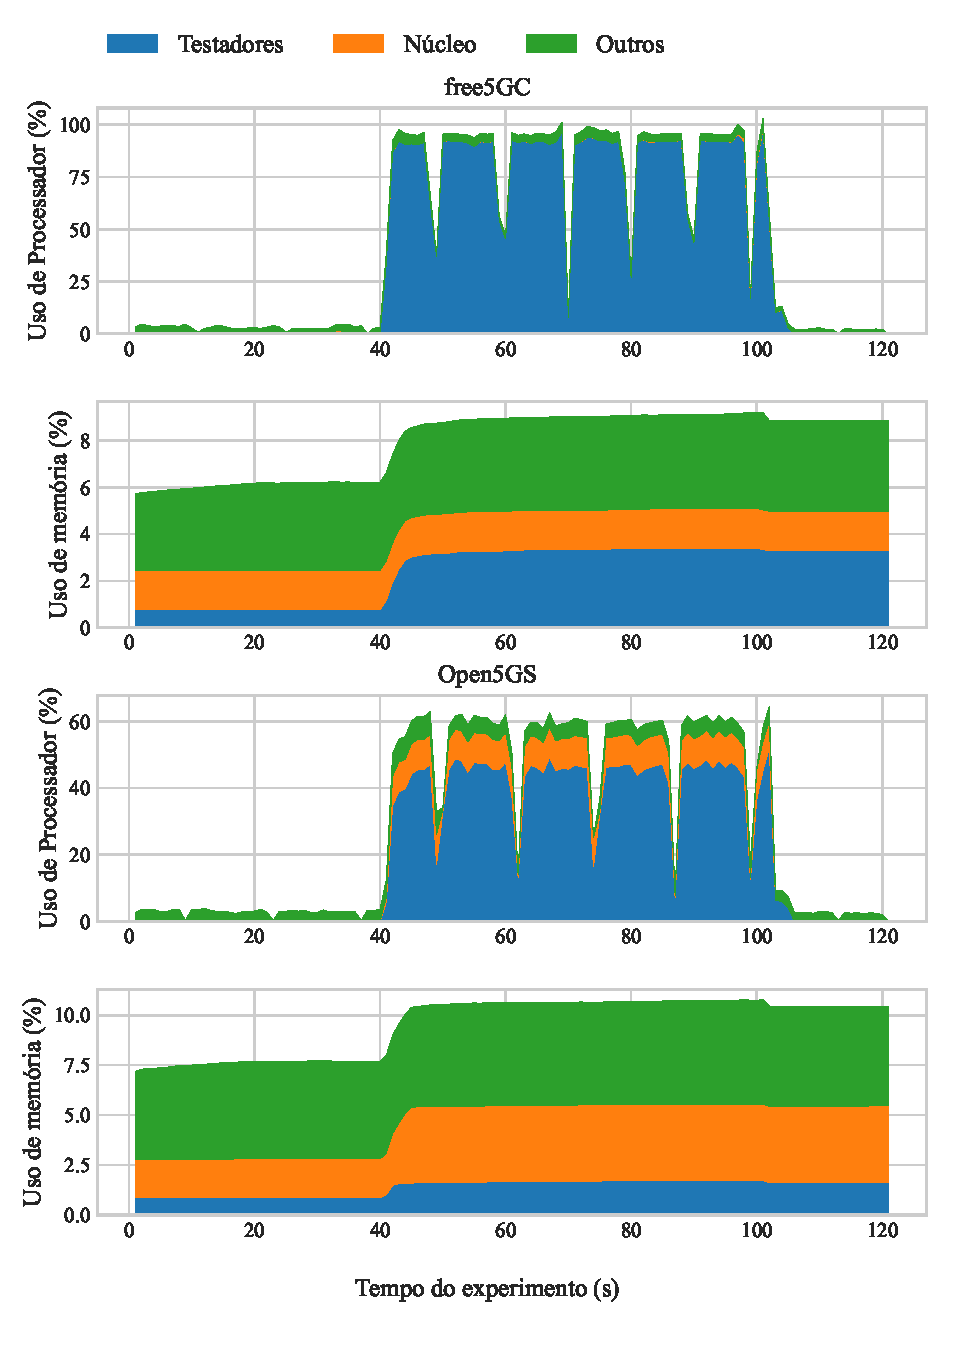
\includegraphics[width=0.95\textwidth]{TG2/Chapters/DataAnalysis/Figures/EXP2-IPERF-RES-10gNB-12C-8GB.pdf}
    \caption{Uso de processador e memória RAM para o experimento de desempenho de plano de dados com 10 UEs conectados}
    \label{fig:exp2_10gnb_12c}
\end{figure}

É possível observar que o uso médio de processador durante a execução desse experimento foi de 95,57\% para o núcleo \textit{free5GC}, com poucos picos de uso atingindo os 100\%.
Do total de uso de processador, 91,87\% do uso é representado pelos testadores e UEs realizando os testes.
O uso de processador médio do núcleo \textit{free5GC} durante a execução do experimento foi de 0,03\%.
Isso demonstra que o núcleo de rede 5G utiliza poucos recursos de processador para realizar o gerenciamento do plano de dados dos UEs conectados.

Em relação ao núcleo \textit{Open5GS}, que não é otimizado para o gerenciamento do plano de dados de múltiplos UEs em paralelo, o uso de processador médio total durante a execução do experimento foi de 59,59\%.
O total de uso de processador durante a execução de experimento é dividida principalmente entre as instâncias do testador e o núcleo da rede 5G, com o testador representando 45,95\% do uso do processador e o núcleo representando 8,96\%.
A redução de uso de processador pelas instâncias do testador e UEs em relação ao experimento executado com o núcleo \textit{free5GC} é explicada pela baixa largura de banda disponível pelo \textit{Open5GS}.

Uma possível explicação desses resultados é que o núcleo \textit{free5GC} provavelmente utiliza paralelização para gerenciar o processamento do plano de dados dos UEs.
Isso provavelmente justificaria a facilidade em escalar a quantidade de UEs conectados reduzindo sutilmente o desempenho individual dos UEs.
Por outro lado, o núcleo \textit{Open5GS} não apresenta o mesmo comportamento.
De acordo com os resultados, o núcleo utilizou 8,96\% do total de processamento disponível na máquina virtual.
Isso é equivalente a um pouco mais que a capacidade de um núcleo do processador disponível.
Possivelmente, este núcleo não está otimizado para paralelizar o processamento do plano de dados quando múltiplos UEs estão conectados.
Isso explicaria o baixo desempenho observado nos resultados do núcleo \textit{Open5GS}.

Ao observar o uso de recursos de processador para a máquina virtual com 4 núcleos virtuais de processador e 4 GB de memória RAM, é possível explicar a queda de desempenho para o plano de dados do núcleo \textit{free5GC} após os testes com mais de 4 UEs simultâneos.
A Figura \ref{fig:exp2_4gnb_4c} representa os gráficos de uso de processador e memória RAM para uma execução do experimento de desempenho do plano de dados 

\begin{figure}[H]
    \centering
    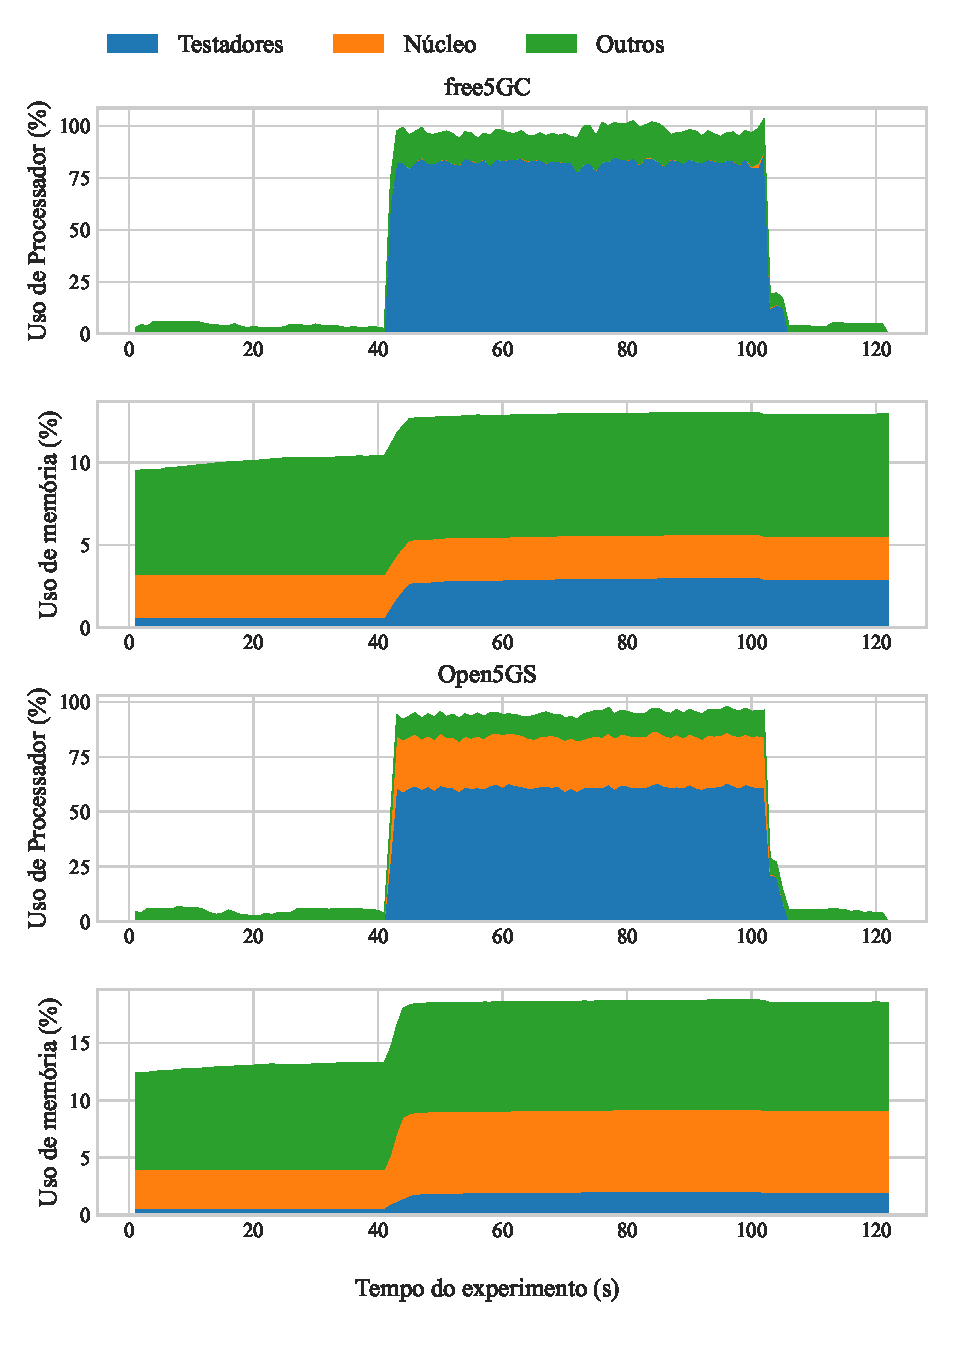
\includegraphics[width=0.95\textwidth]{TG2/Chapters/DataAnalysis/Figures/EXP2-IPERF-RES-4gNB-4C-4GB.pdf}
    \caption{Uso de processador e memória RAM para o experimento de desempenho de plano de dados com 4 UEs conectados}
    \label{fig:exp2_4gnb_4c}
\end{figure}

É possível observar que o uso do processador para a execução de quatro UEs conectados e utilizando o plano de dados do núcleo de rede 5G \textit{free5GC} está muito próximo de 100\%, atingindo o uso máximo do processador em diversos momentos.
Dessa forma, é possível perceber que o máximo de UEs simultâneos que essa configuração de máquina virtual suporta são quatro.
Para quantidades superiores a quatro UEs simultâneos, a redução de desempenho do plano de dados é explicada devido ao chaveamento necessário realizado pelo sistema operacional para gerenciar os diversos processos executando em paralelo.




% Livro sobre análise de dados:
% https://app.minhabiblioteca.com.br/reader/books/9788584291434/pageid/28


\chapter{Considerações finais e trabalhos futuros}
\label{chap:conclusion}
O presente trabalho atinge a proposta inicial, desenvolvendo uma ferramenta para testes de desempenho de redes móveis 5G de código aberto, além de avaliar o desempenho em dois distintos cenários com duas implementações de núcleo 5G existentes.
As descobertas e limitações encontradas podem ser úteis para o desenvolvimento dos núcleos. Da mesma forma, essa ferramenta pode ser utilizada para avaliar outros núcleos não testados no presente trabalho.

Este trabalho apresenta duas principais contribuições teóricas. A primeira é com relação aos testes de desempenho, principalmente sobre redes móveis.
A implementação do módulo de execução dos testes de desempenho e análise dos dados coletado traz discussões relevantes sobre a utilidade do uso de testes de desempenho durante o desenvolvimento de software.
Essas discussões são de extrema relevância para a área de Engenharia de Software, mostrando que os testes de desempenho ajudam a validar implementações de software para operarem de maneira correta sobre alta carga de trabalho.

A segunda contribuição teórica deste trabalho é em relação à estabilidade das atuais implementações de código aberto de núcleos de rede 5G.
As três implementações avaliadas possuem grandes limitações em relação ao desempenho em escala, tornando sua implantação em redes reais inviável neste momento.
Esse trabalho demonstra que a implementação OAI, sendo a menos madura delas, não conseguiu rodar nenhum dos testes de desempenho devido a suas limitações.
Por outro lado, as outras duas implementações avaliadas apresentam diversas limitações que fizeram com que o módulo de testes de desempenho desenvolvido fosse adaptado para funcionar sobre as limitações encontradas e descritas no decorrer do trabalho.

Este trabalho também possui contribuições práticas, ao desenvolver um módulo para ser acoplado no testador \textit{my5G-RANTester} de núcleos 5G.
Este módulo está disponível no repositório de código do projeto PORVIR-5G e é aberto para a comunidade.
Dessa forma, é possível utilizar a implementação do testador disponível para realizar testes sobre novas versões das implementações existentes de núcleos 5G e para outras implementações futuras.

Este trabalho possui algumas limitações.
Dentre elas, pode-se citar as limitações dos núcleos testados, fazendo com que os testes em escala fossem limitados a uma menor quantidade de UEs se registrando, estabelecendo uma sessão PDU e trafegando dados.
Outra limitação relevante é em relação à execução do testador na mesma máquina virtual onde o núcleo foi executado.
Ao executar todo o ambiente de testes na mesma máquina que está sendo executado o núcleo da rede 5G, os recursos de hardware disponíveis são divididos entre os processos em execução.
Dessa forma, o uso de memória RAM e processador pelo testador para gerenciar as diversas conexões de UEs e pelos UEs para executar testes de largura de banda reduz a quantidade de recursos disponíveis para o núcleo, afetando o seu desempenho.

O presente trabalho abre oportunidades para futuros experimentos em relação ao desempenho de núcleos de redes 5G.
Um exemplo seria o teste sobre outras implementações de núcleos de redes 5G de código aberto não avaliadas no presente trabalho.
Outro tópico para pesquisas seria avaliar o desempenho de implementações comerciais de núcleos de redes 5G.
Além disso, pode-se utilizar a implementação atual do testador, executando testes sobre ambientes de fácil escalabilidade, permitindo executar o testador em uma máquina virtual separada da máquina que está executando o núcleo a ser testado.
Dessa forma, o uso de recursos do testador não deve afetar a disponibilidade de recursos para o núcleo, tendo resultados mais relevantes em relação ao funcionamento da implementação em teste.


% e aqui vai a parte principal
%
% \chapter{Estado da arte}
% \chapter{Mais estado da arte}
% \chapter{A minha contribuição}
% \chapter{Prova de que a minha contribuição é válida}
% \chapter{Conclusão}

% referencias
% aqui será usado o environment padrao `thebibliography'; porém, sugere-se
% seriamente o uso de BibTeX e do estilo abnt.bst (veja na página do
% UTUG)
%
% observe também o estilo meio estranho de alguns labels; isso é
% devido ao uso do pacote `natbib', que permite fazer citações de
% autores, ano, e diversas combinações desses

\bibliographystyle{abntex2-alf}
\bibliography{TG2/references,TG2/refs-3gpp,TG2/refs-web}

\end{document}
